\documentclass[sigconf]{acmart}
%\usepackage{threeparttable}
\usepackage{appendix,float}
% \usepackage{todonotes}
\usepackage{array}
\usepackage{subcaption}
\usepackage{graphicx}
\usepackage{tikz}
\usepackage{wrapfig}
\usepackage{titlesec}
\usetikzlibrary{calc, positioning, arrows.meta}
\usetikzlibrary{decorations.pathreplacing} 
\titlespacing*{\section}{0pt}{0.5ex plus 1ex minus .2ex}{0.3ex plus .2ex}

\AtBeginDocument{%
  \providecommand\BibTeX{{%
    \normalfont B\kern-0.5em{\scshape i\kern-0.25em b}\kern-0.8em\TeX}}}

\copyrightyear{2025} 
\acmYear{2025} 
\setcopyright{cc}
\setcctype{by}
\acmConference[DESTION '25]{The 7th Workshop on Design Automation for CPS
and IoT }{May 6--9, 2025}{Irvine, CA, USA}
\acmBooktitle{The 7th Workshop on Design Automation for CPS and IoT
(DESTION '25), May 6--9, 2025, Irvine, CA, USA}
% \acmPrice{15.00}
\acmDOI{10.1145/3722573.3727830}
\acmISBN{979-8-4007-1604-1/2025/05}
\makeatletter
\renewcommand{\@authorfont}{\normalfont\large}
\makeatother
\begin{document}
\title{Autonomous Cybersecurity Testbed for Operational Technology Networks}
% \author{Akhilesh Raj,Harsh Vardhan,Himanshu Neema,Sanjana Das,Ajay Chhokra,Daniel Balasubramanian}
% \email{{akhilesh.raj,harsh.vardhan,himanshu.neema,ajay.d.chhokra,sanjana.das,daniel.a.balasubramanian}@vanderbilt.edu}
% \affiliation{%
%   \institution{Vanderbilt University}
%   \city{Nashville}
%   \state{TN}
%   \country{USA}
% }
% \renewcommand{\shortauthors}{Raj, A., et al.}


\author{{Akhilesh Raj, Sanjana Das, Harsh Vardhan, Himanshu Neema, Ajay Chhokra, Daniel Balasubramanian}}
\email{akhilesh.raj, sanjana.das, harsh.vardhan, himanshu.neema, ajay.d.chhokra, daniel.a.balasubramanian@vanderbilt.edu}
\affiliation{%
  \institution{Vanderbilt University}%
  \city{Nashville}
  \state{TN}
  \country{USA}
}
\renewcommand{\shortauthors}{Raj, A., et al.}


\section*{Abstract}
In the ongoing era of Fourth Industrial Revolution (4IR), where the manufacturing and industrial processes are being integrated with information technologies including Artificial Intelligence (AI), advanced testbeds are a must to ensure an error-free, scalable and gradual transition. The network-integrated Operational Technology (OT) used in manufacturing industries also requires advanced testbeds to test and evaluate cybersecurity agents deployed to mitigate adversarial attacks.
In this paper, we describe a testbed designed for testing and evaluating attack-resilient network agents, also known as blue agents. Using open-source software stacks and network protocols, we develop an easy-to-deploy, OpenStack-based network emulator that closely emulates industrial use cases. We also demonstrate the utility of this testbed by initiating various attack types that lead to OT plant instability. The various stages of the experiments, leading to this instability, can be detected and recorded using the measurement tools available within the testbed.

% \keywords{networked co-simulation, cyber-physical systems, system-of-systems, high-level architecture, modeling and simulation}
\keywords{Operational Technology, OT-networks, emulation, simulation, CPS, Cybersecurity}


\maketitle
\section{Introduction}
\begin{figure}[htb]
    \centering
    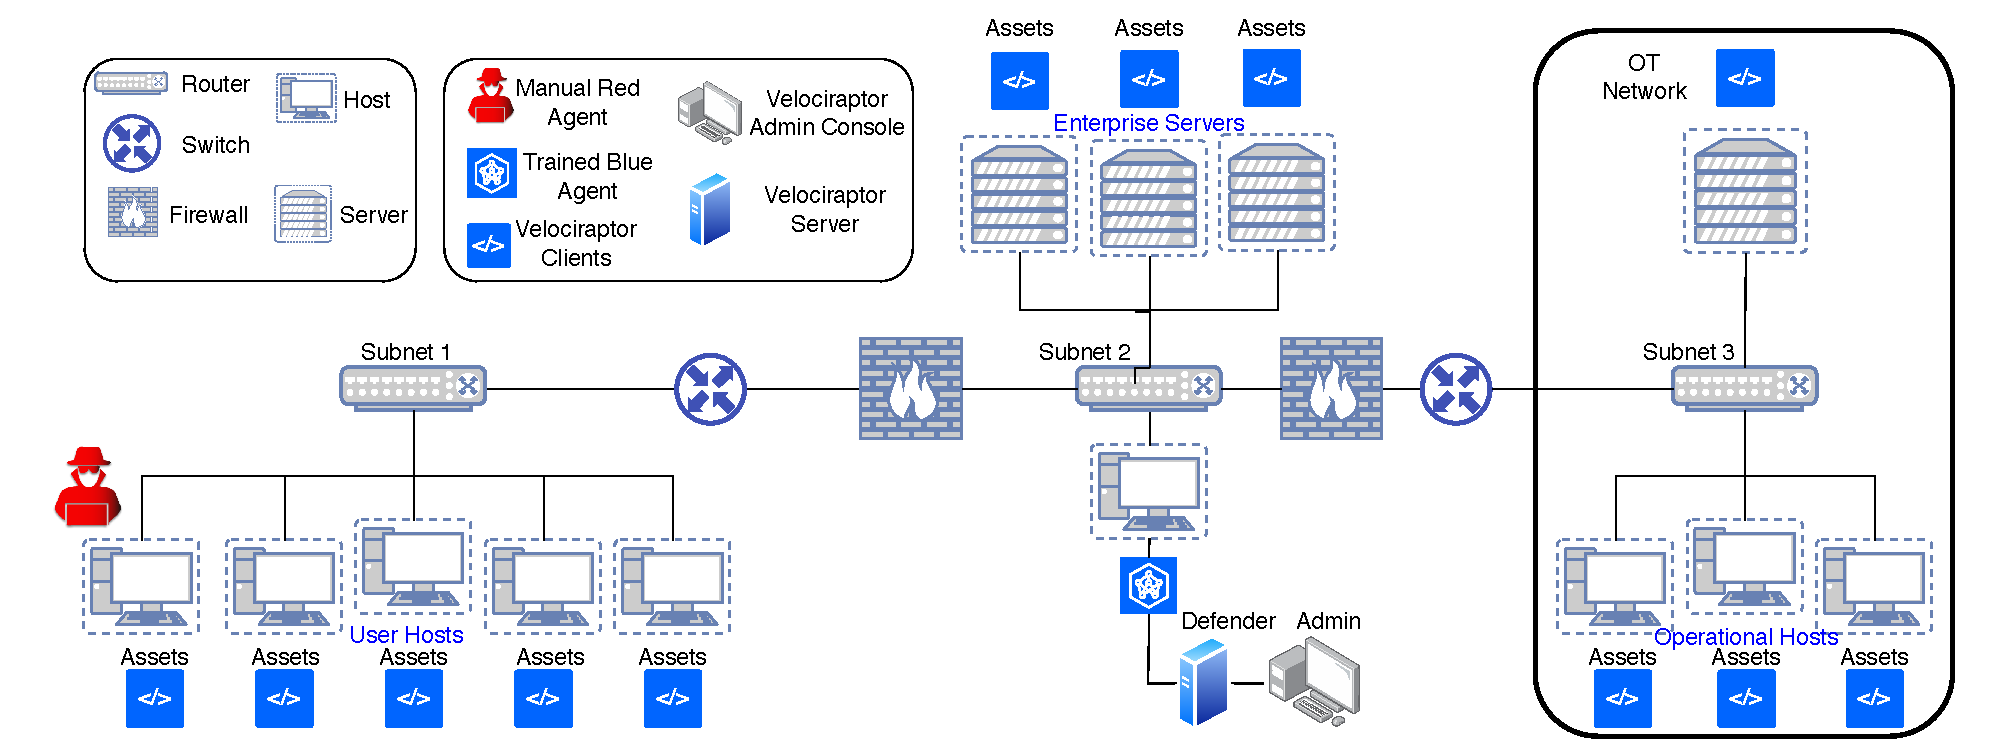
\includegraphics[width=\linewidth,trim={0cm 0cm 0cm 0cm}, clip]{Figures/cage2.pdf}
    \caption{Schematic of the enterprise CAGE-2 network topology with embedded OT network.}
    \label{fig:Enterprise_Network}
\end{figure}
Operational Technology (OT) networks are critical infrastructure systems responsible for controlling physical processes in industries such as manufacturing, energy, transportation, and utilities \cite{negi2024towards} . These networks integrate hardware and software systems, including Supervisory Control and Data Acquisition (SCADA), Programmable Logic Controllers (PLCs), and Distributed Control Systems (DCS), to ensure the smooth operation of industrial machinery and processes. However, with the convergence of OT and Information Technology (IT) systems with increased digitalization and Industry 4.0 initiatives, OT networks have become a prime target for Cyber threats in recent time \cite{knapp2024industrial} \cite{zaid2024emerging}. Unlike traditional IT systems, OT networks face unique cybersecurity challenges due to their legacy systems, real-time operational requirements, and the high economic loss incurred during its downtime or failure. Cybersecurity in OT networks, therefore, focuses on safeguarding critical infrastructure from threats such as malware, ransomware, and state-sponsored attacks, ensuring the continuity, safety, and reliability of essential services.
Attackers target the OT-networks through methods like social engineering, exploiting vulnerabilities in IT components, malware injection, supply chain attacks, and insecure remote access, with spear phishing and the Stuxnet worm as notable examples \cite{stojanovic2020apt}.
These breaches not only compromise sensitive OT systems but also result in significant financial losses, as highlighted in IBM's report \cite{IBM}.
%indicating the loss of millions of dollars per data breach.
%average cost of a data breach at \$4.88 million—a 10\% hike from the previous year—and the Colonial Pipeline ransomware attack, which caused a direct ransom payment of \$4.4 million and significant disruptions.
Moreover, the report also highlights the steep costs associated with downtime in OT,
%(\textasciitilde\$260K/hr.),
emphasizing the critical need for robust OT cybersecurity to prevent such expensive and operationally disruptive incidents. Manual efforts for cybersecurity are time-consuming and error-prone, which necessitates the use of automated cyber agents. However, before deploying these cyber agents must be thoroughly evaluated on their performance because the behavior of the agents could be very different in emulation (that mirrors the real-world use-case) as opposed to in pure network simulation (where these agents are typically trained). This requires a general-purpose, configurable testbed to evaluate cyber agents for the OT networks. Such testbeds are currently lacking.

In this paper, we describe a highly configurable emulation testbed for evaluating cyber agents in the OT networks.
%To curb this threat to the industries, {cybersecurity-agents} or cyber-agents are deployed within the network with diverse objectives.
Our testbed enables realistic evaluation of these cyber agents, thereby bypassing the expensive and rather potentially dangerous real world testing. The proposed emulation environment, hosted on openstack, can be integrated as a subnet of a larger network topology and in its present form, also provides to the users, a programmable interface that is vulnerable to attack. The OT use cases deployed using this testbed, consists of power grid (utility) and chemical plant (industry) environments, whose controllers rely on their respective OT networks for information exchange and control. The visualization of the plant operations along with the information using SCADA, helps users analyze the state of the plant at any time, thereby understanding the impact of an action taken by the agent on the OT network. In addition, we showcase the application of these features within the proposed testbed through the execution of basic network and host attacks, and we observe the ensuing impact on the electrical grid and chemical processing facilities.


The rest of this paper is organized as follows - Section \ref{sec:related} details related work by reviewing the characteristics of existing testbeds and identifies the basic requirements for the testbed.
%states the characteristics of various testbeds we have identified as a potential {cyber-agent} testbed also highlighting some of the requirements a testbed offers.
Section \ref{sec:architecture} describes the overall architecture of our testbed, its design and integration methods. Section \ref{sec:casestudy} presents two case studies covering the attacks on power grid and chemical plant environments and underlines
%discusses the case study using attacks underlining
the limitations that we have identified. Section \ref{sec:conclusion} presents potential future extensions and concluding remarks.



\section{Related Work}
\label{sec:related}
Cybersecurity Testbeds designed for AI testing and evaluation, particularly within the OpenAI Gym environment, can be broadly classified into simulation and emulation testbeds. On the simulator side, there are tools like \textit{CyberBattleSim (CBS)}, \textit{Network Attack Simulator (NASim)} and \textit{CybORG}. 

On the emulator front, the testbeds NASimEmu \cite{janisch2023nasimemunetworkattacksimulator} and  CyGIL \cite{li2021cygil} provide the AI training and testing of cybersecurity agents. 
CyGIL \cite{li2021cygil} employs a stateless environment architecture and integrates the MITRE ATT\&CK framework to create a high-fidelity training environment. It features an abstracted interface that facilitates reinforcement learning (RL) training to focus on specific advanced persistent threat (APT) profiles. It also assumes that it has red team coordination and control (C2) infrastructure with centralized coordination and distributed execution. 
Currently, CyGIL only supports testing red agents. CyGIL relies on CALDERA to enable red team emulation
using the MITRE ATT\&CK framework that encompasses and analyses reported cyber-attack tactics, techniques, and procedures (TTPs). NaSimEmu relies on metasploit for enabling red team control and attack execution. To that end, we enhance the Reinforcement Against Malicious Penetration by Adversaries in Realistic Topologies (RAMPART) \cite{10564815} project, which already supports these attributes, by integrating the proposed testbed.


% Latter is the end goal of the larger Reinforcement Against Malicious Penetration by Adversaries in Realistic Topologies (RAMPART) \cite{10564815} project, of which this testbed is a part of. 
Presently, these platforms lack the use-cases where the observables for the agents are host or application-specific. In this paper, we focus on integrating a real-world OT emulator, providing users with access to emulation-generated measurements that enhance network agents' decision-making capabilities. By developing the proposed emulator for research communities to test and evaluate their reinforcement learning agents, we ensure:
% \vspace{-0.5cm}
\begin{itemize}
    \item supported software and hardware stacks,
    \item a state of the art network infrastructure facilitating customizable user/ application interface and interactions,
    \item a generic and scalable network topology with provisioned host images supported to run the use cases,
    \item a state of the art emulator capable of recreating OT plant behavior with OT-specific observations.
\end{itemize}
% \vspace{-1cm}


% % \section{Network Emulator Requirements}
% \label{sec:requirements}
% The purpose of this testbed is to provide researchers and developers a platform for testing and evaluation of resilient reinforcement learning agents. 
By developing the proposed emulator for research communities to test and evaluate their reinforcement learning agents, we ensure:
\begin{itemize}
    \item supported software and hardware stacks,
    \item a state of the art network infrastructure facilitating customizable user/ application interface and interactions.
    \item a generic and scalable network topology with provisioned host images supported to run the use cases mentioned in this paper.
    \item a state of the art emulator capable of mimicking real-world OT plant behavior capable of providing to the users, OT-specific observations.
\end{itemize}
% Beyond these capabilities, the OT network must reliably mimic real-world OT plant behavior. To support this, our emulation environment offers reconfigurable OT use cases for a power grid and a chemical plant, along with built-in attack scripts and demonstration scenarios.




\section{Integration Architecture}
\label{sec:architecture}
As discussed in Section \ref{sec:related}, this paper focuses on the proposed testbed as an integral part of the RAMPART cyber agent training workflow. Although we confine our discussion here to the OT networks, it is important to note that the integration architecture and the base images used are inherited from the RAMPART network topology or the $CAGE-2$ topology as shown in Figure \ref{fig:Enterprise_Network}. Moving forward, the larger network that the OT network is integrated into will be referred to as the enterprise network.

In this testbed, we deploy two specific OT use cases, a Power Grid and a Chemical Plant. 
% \begin{itemize}
%     \item \textbf{Power Grid} - hosted as a single host-only-network within the enterprise network,
%     \item \textbf{Chemical Plant} - hosted as a subnet consisting of three hosts within the enterprise network.
% \end{itemize}
Using the support from different software modules we replicate the real-world dynamics of a power grid and a chemical plant on OpenStack hosts, which makes it a realistic testbed for testing and evaluating cyber agents for OT networks. OpenStack is an open-source cloud computing platform that provides a set of software tools for building and managing cloud computing environments.
% It enables researchers and businesses to deploy virtual servers and other resources such as storage and networking services, enabling them to create scalable and flexible cloud infrastructure. OpenStack is designed to facilitate the widespread adoption of cloud services by being hardware-agnostic and providing a high degree of control over the environment. It provides a user friendly interface to design network topologies and host devices connected to them along with the required peripherals.
As the enterprise network with the \textit{CAGE-2} \cite{kiely2023autonomousagentscyberdefence} topology is built on OpenStack, we conformed to the \textit{CAGE-2} integration rules for building the OT network.
\subsection{Power Grid}
This use case replicates a real-world scenario of a smart grid consisting of three substations and a power house as shown in the Figure \ref{fig:powergrid}. This example underlines the importance of securing OT networks in smart grids. The working of the power grid emulator is governed by three important components; all installed on a single host machine connected to the enterprise network.
\begin{figure}[!ht]
    \centering
    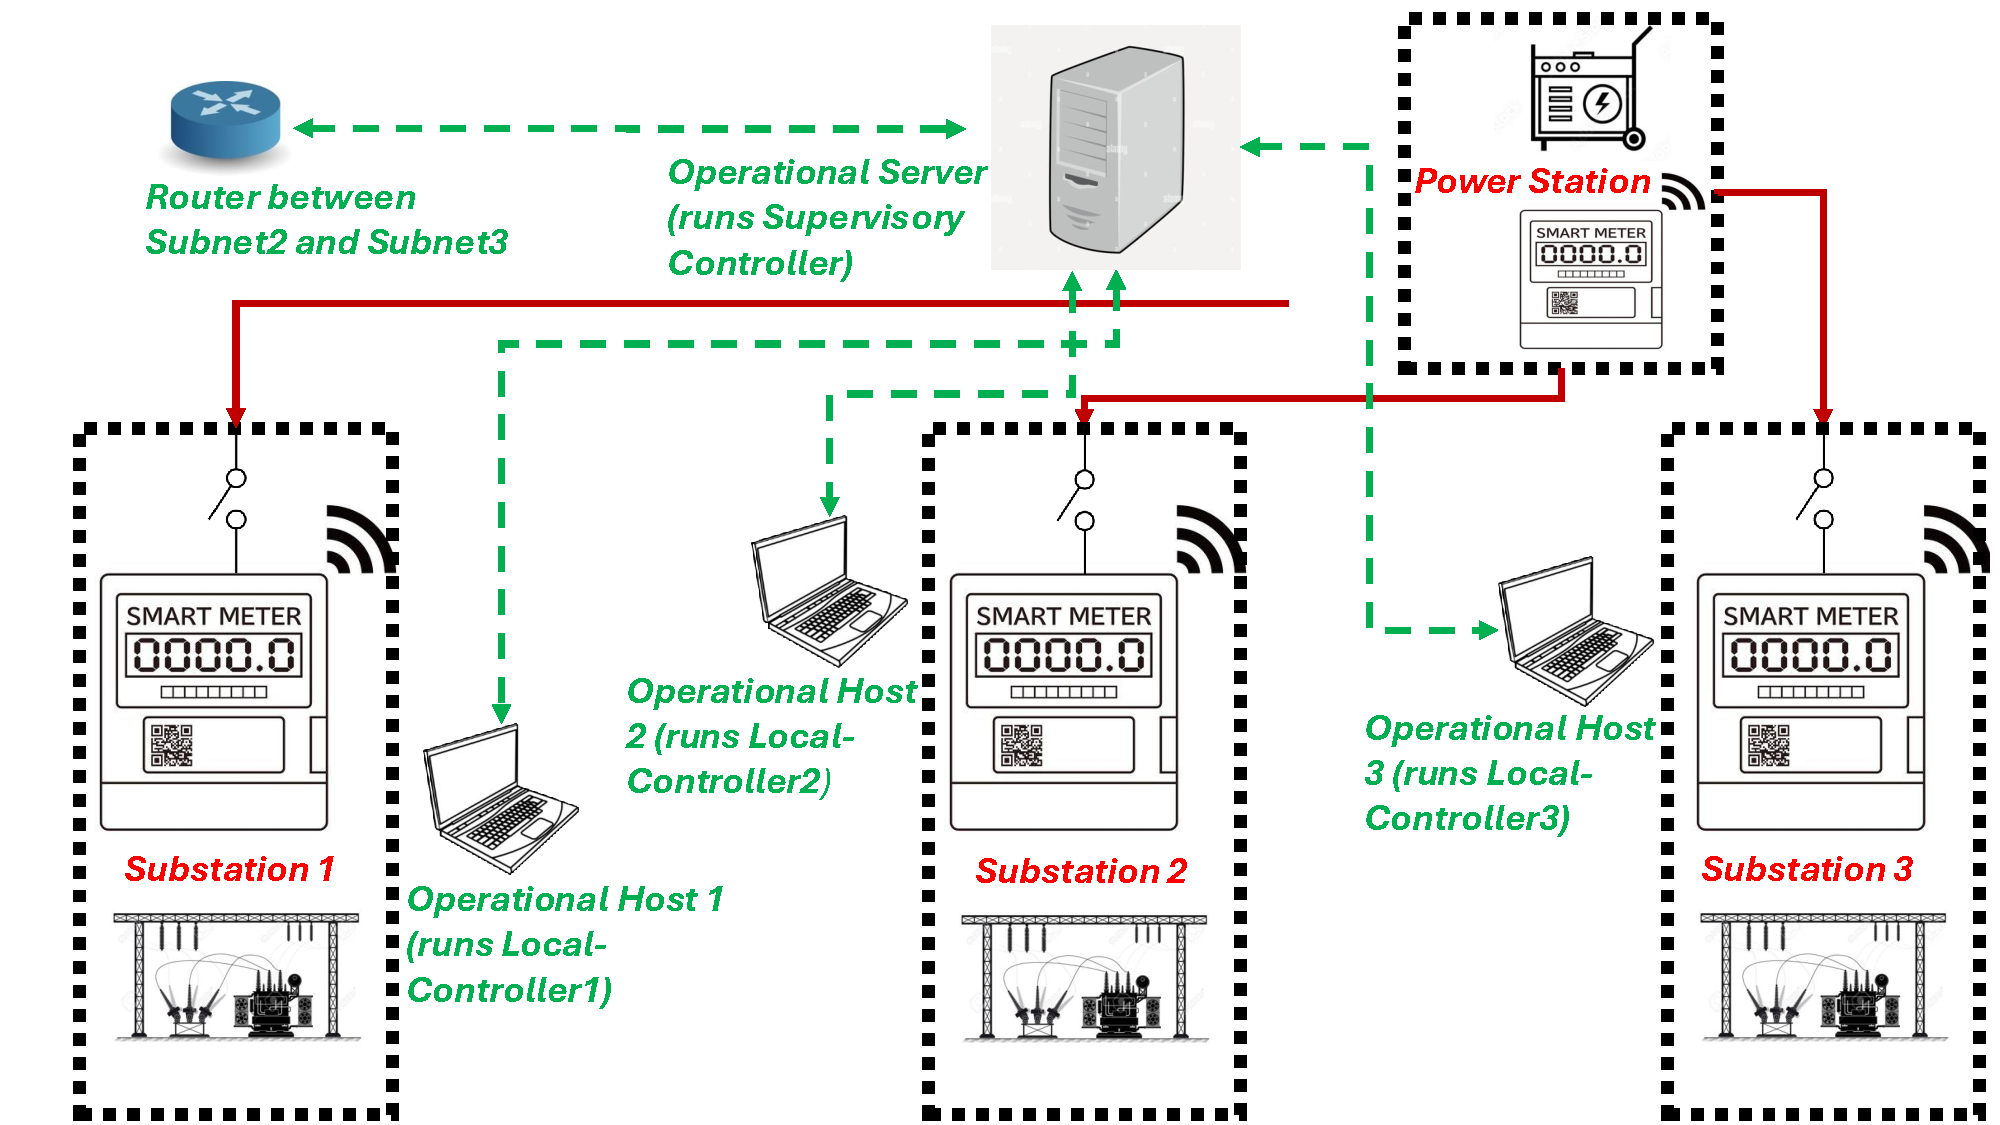
\includegraphics[width=\linewidth, trim=0.25cm 0.5cm 0cm 0cm]{Figures/powergridotnw_new.pdf}
    \caption{Block diagram depicting the use of OT networks in Smart Grids and the underlying hardware-software integration. The red line represents the Power grid operations (GridLAB-D emulations) and the green corresponds to the OT networks (Mininet emulation).}
    \label{fig:powergrid}
% \vspace{-0.6cm}
\end{figure}
\subsubsection{GridLAB-D} It is an advanced power distribution system simulation and analysis tool, aiding designers, operators, and utilities in optimizing energy technologies \cite{chassin2014gridlab}. Developed by the U.S. Department of Energy at Pacific Northwest National Laboratory, it features cutting-edge modeling techniques and distribution automation models using a variety of modules designed for a variety of use-cases. We use this software as the simulation platform replicating a real-world power grid system. In the real-world micro-grid and smart-grid scenarios, the regulators and controllers used to maintain the desired power and performance metrics rely on the OT network for sensing and actuation. We recreate this behavior using GridLAB-D in the server mode. The server mode of GridLAB-D (v4.3) enables the OT network to communicate with the grid using standard TCP/IP protocols.
% We use the GridLAB-D v4.3 for our experiments.
Here we highlight some of the key components of GridLAB-D used in this testbed:
\begin{itemize}
    \item \textit{Generator} object hosts a variety of power sources with control including simple solar models, wind turbine models, and battery control models. 
    % This module helps create an open environment for distributed generation, where users can create their own models, including control algorithms.
    \item \textit{Meters} are general purpose energy and power meters. These are useful for time-varying simulations with recorder objects attached for data collection.
    % GridLAB-D's normal output methods (.xml, .txt) will only record the final time-step of a system, so for time varying systems a recorder and meter are needed to track power and energy, as well as voltage and current.
    \item \textit{Recorder} provides the ability to collect a recording of one or more properties of an object with user-defined sampling interval, triggers, and other properties.
    \item Switch object serves as the simple electrical disconnect device. This object acts as an actuator in the testbed.
    \item \textit{Overhead lines}  provides configurable (resistance, length, material etc.) object as connecting components.
    \item \textit{Load} is a configurable object to represent a generic power sink with phases, voltage, and current parameters.
    % \item Zip-Load : The ZIPload model is designed to provide a means to access the Residential class at a fundamental level and from a power engineer perspective. Users can design and connect the ZIPload to environment variables, that changes the power consumption of the load based on the weather data that gives it more realistic sim environment. 
\end{itemize}

\subsubsection{Mininet} It allows emulating simplified, scaled-down versions of real-world computer networks, often used for educational or experimental purposes \cite{10.1145/1868447.1868466}. It enables users to emulate network topologies, test network protocols, and study network behavior in a controlled environment, facilitating learning and research in networking concepts. In our setup, a single Mininet instance hosts the OT network, comprising four nodes. One node runs the supervisory controller (\textit{SC}) and the other three run the local controllers (\textit{LCs}). These controllers communicate with the \textit{GridLAB-D} server to monitor and report relevant system metrics.

% \vspace{-0.1cm}

\subsubsection{Two-Level Controllers} As shown in the Figure \ref{fig:powergrid}, the OT network consists of one Operational Server (OS) running the \textit{SC} and three operational hosts (OH) running the \textit{LCs} connected through a router. In the current setup, all nodes in the OT network are homogeneous, with their responsibilities and capabilities determined by the controllers running on them. These controllers play a crucial role in sensing key metrics of the grid and actuating components within the GridLAB-D simulator. Some of the key monitored parameters include three-phase power measurements, substation loads, switch statuses, and triplex meter readings.

The \textit{SC} is responsible for distributing power efficiently while preventing generator overload, based on the requirements and priority levels received from the \textit{LCs}. It continuously monitors the total power consumption across the three substation loads and generators, ensuring balanced distribution. 
Additionally, the \textit{SC} transmits regulatory information to the \textit{LCs}, enabling them to make informed decisions for localized power management.

The \textit{LCs} periodically collect measurements from GridLAB-D within their assigned scope. Every 5 seconds, they transmit data on future power demand and substation priority levels to the \textit{SC}. Upon receiving regulatory instructions from the \textit{SC}, the \textit{LCs} adjust the power distribution to ensure efficient grid operation.
% \end{itemize}
% The schematic of the power grid integrated with its corresponding network is as shown in the Figure \ref{fig:powergrid}.


Figure \ref{fig:powergrid} shows the schematic of the smart grid OT network consisting of a power grid simulator and the corresponding network.
% The power grid is simulated using GridLAB-D. It replicates the working of a power grid given consisting of a generator and three substations connected using overhead lines and switches. 
The power generator is designed to generate power at a constant voltage and deliver it to the substation through the overhead lines. The substations consist of loads designed to include utilities in the form of loads. These loads can be disconnected from the grid at any time with the help of the switch present at the substations. In the normal mode, the power station delivers the power based on the substation demands and priority levels at a constant voltage. 

In a Smart Grid, the \textit{LCs} at each substation calculate the power demand over predefined time intervals. Additionally, they determine the priority levels of these demands based on the types of loads connected to the substation. While various algorithms can be used to assign priorities, this testbed employs a random number generator to set priority levels for each load. The \textit{LCs} communicate the demand and priority data to the \textit{SC} via the OT network using the TCP/IP protocol. Upon receiving this information, the \textit{SC} re-calculate the power allocation across substations, ensuring that available power is distributed according to priority rankings. If the total requested power exceeds the power station’s capacity, substations with the lowest priority rankings experience a power shortage. If the shortage is severe enough -- meeting or exceeding the demand of lower-priority substations -- some or all of these substations enter islanding mode. 
% In this mode, substations are disconnected from the grid for the remainder of the current interval by opening their corresponding switches. 
The operator can monitor the requests of each of the controllers and the corresponding power allocation through the visualizer present locally at the node. 

% The primary controller can visualize the demand and usage using the visualization tool present locally as shown in the Figure \ref{fig:Visualizer}.
% \begin{figure}[H]
%     \centering
%     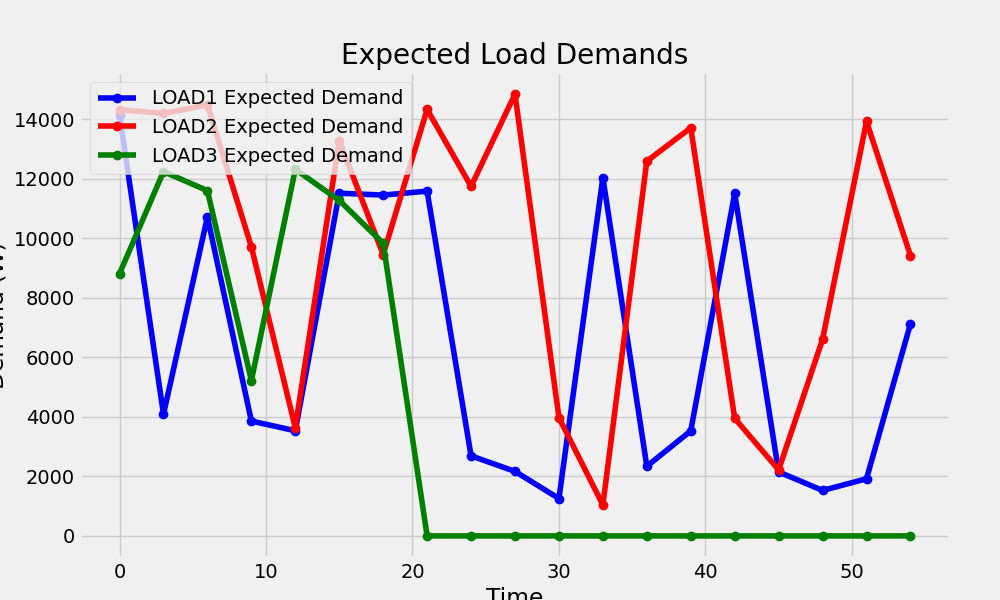
\includegraphics[width=\linewidth]{Figures/expected_load_demands_lc3_dos.png}
%     % \todo{Wrong figure.}
%     \caption{Live Visualization of the power generated and the power consumed by each load.}
%     \label{fig:Visualizer}
% \end{figure}


% \begin{figure}
%     \centering
%     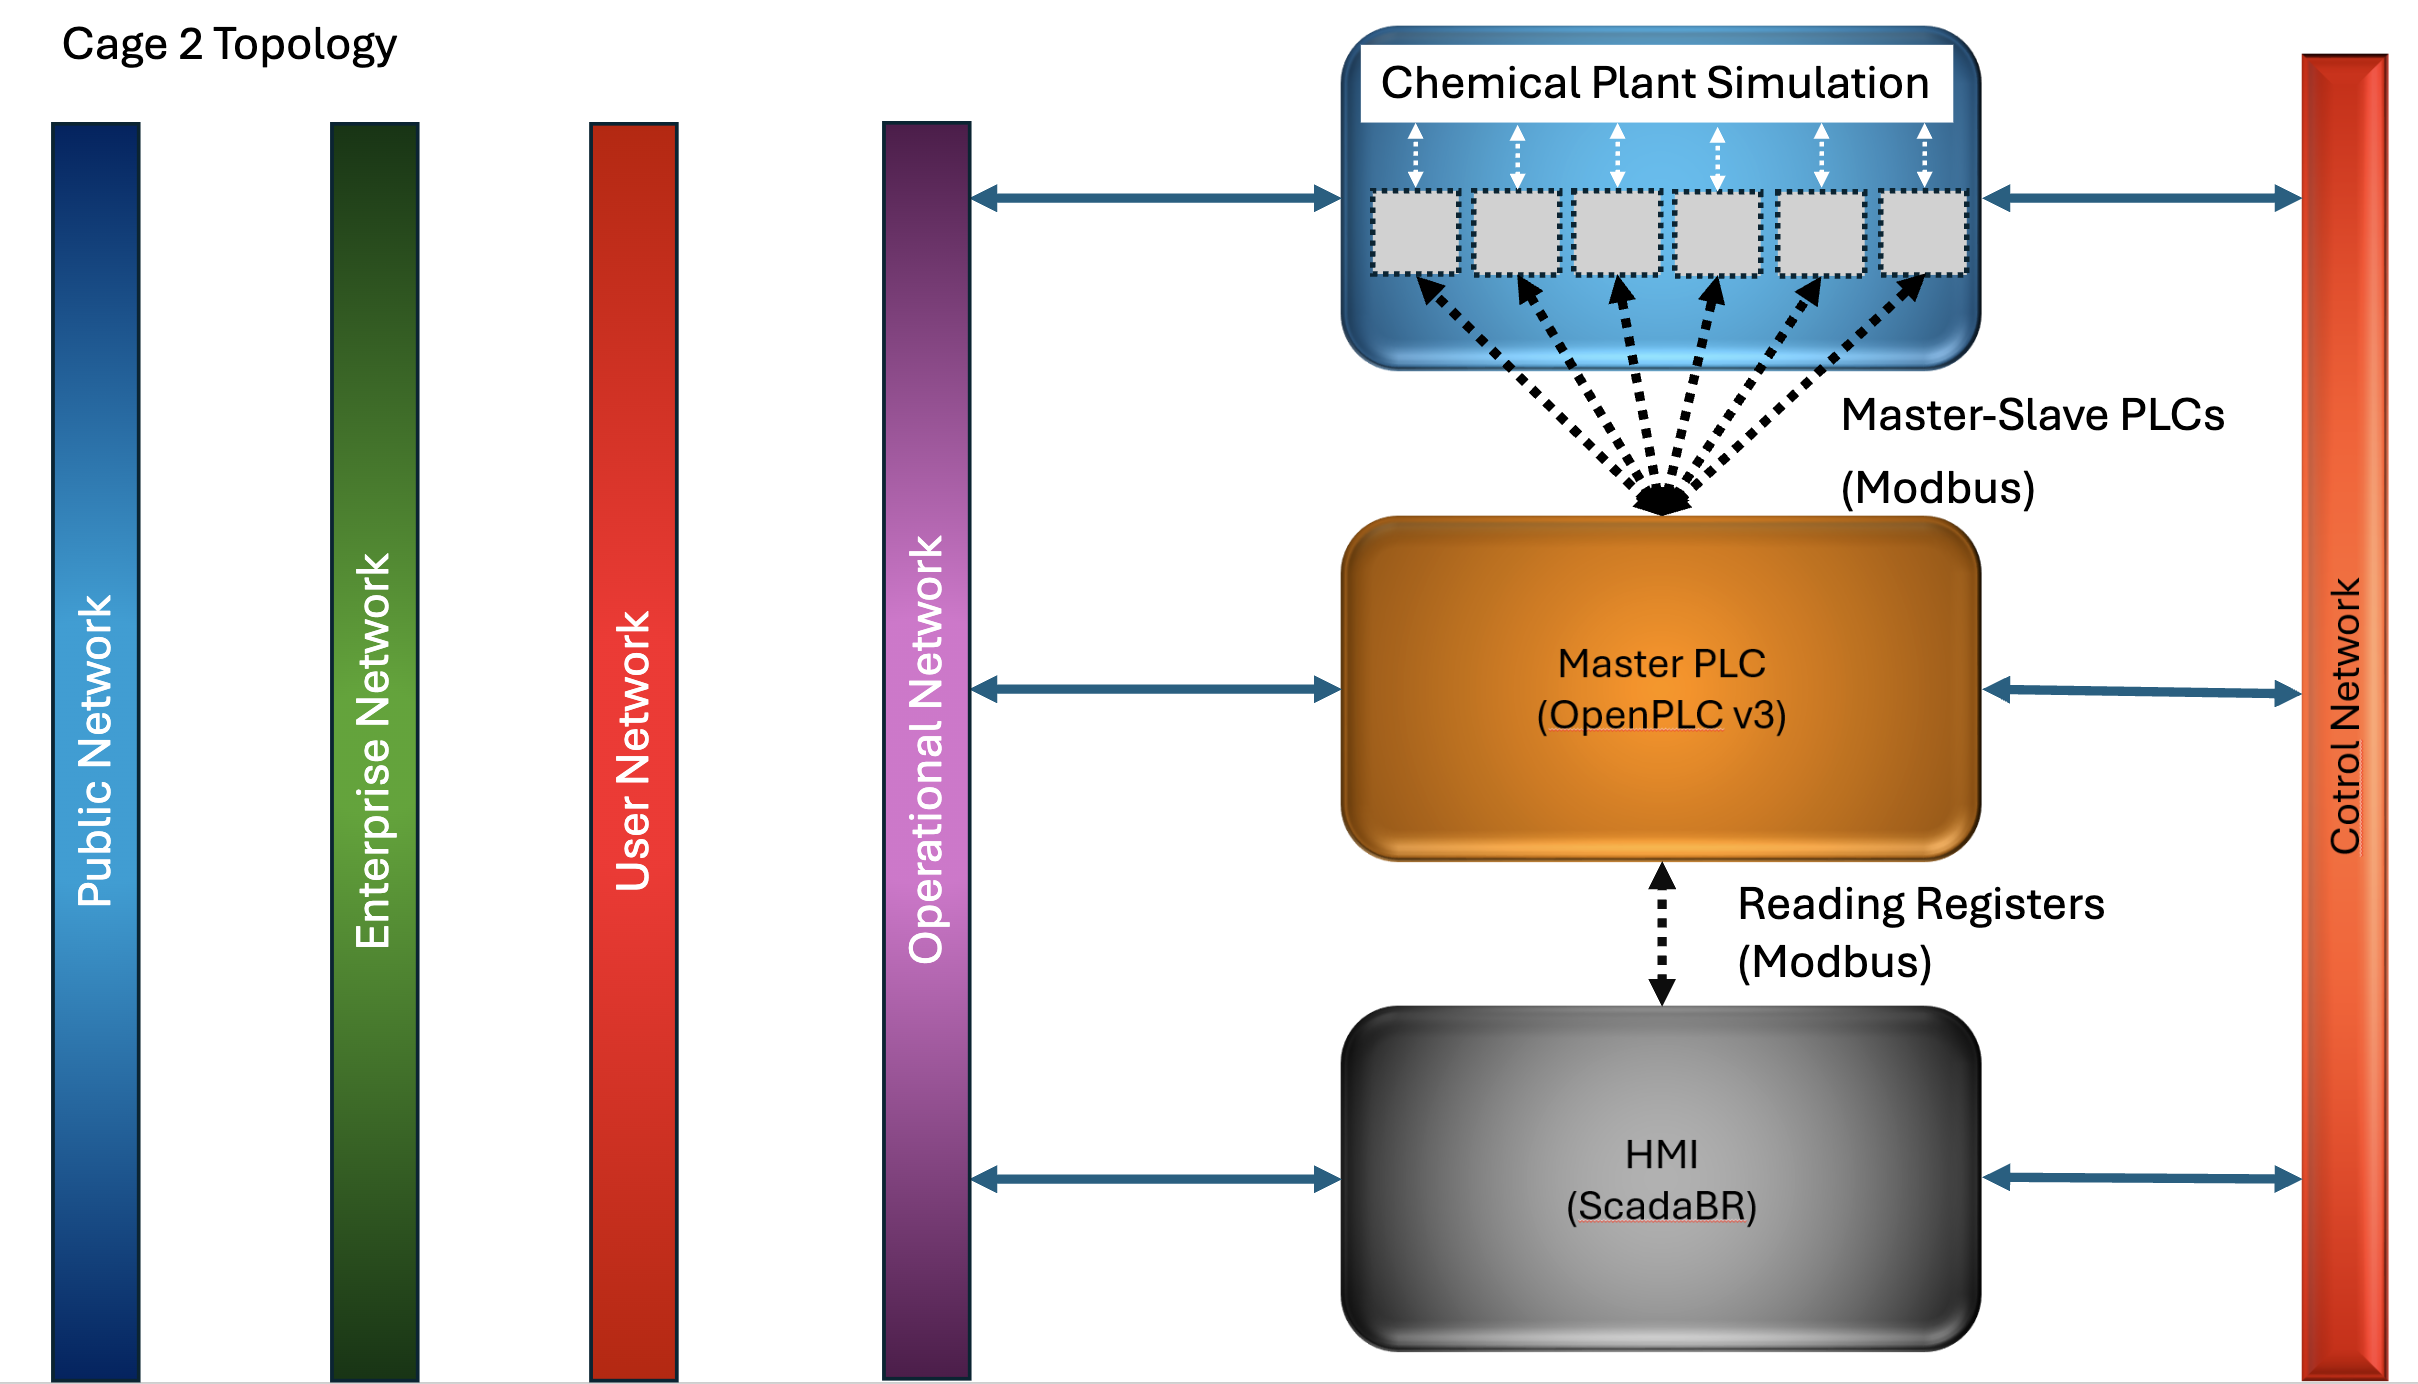
\includegraphics[width=\linewidth]{Figures/ChemicalPlantNW.png}
%     \caption{A schematic of the Chemical plant OT network depicting the }
%     \label{fig:Chemical Plant}
% \end{figure}

% \vspace{-0.2cm}
\subsection{Chemical Plant}
The Chemical Plant Workflow is the adaptation of the testbed used for the experiments related to Industrial Control Systems (ICS) by David et al. \cite{formby2018lowering}. The main components of this OT workflow are:
\subsubsection{Graphical Realism Framework For ICS (GRFICS):} We use GRFICS ~\cite{formby2018lowering} for developing a use-case by hosting its different components on the openstack host machines.
The GRFICS was designed as a modular system 
for customization and scalability, using standard ICS network protocols to connect elements like Human Machine Interface (HMI), Programmable Logic Control (PLC), and Input/Output (I/O) modules, and permits the interchanging of these components with actual ICS devices. It integrates physical process simulation with 3D visualization and the I/O module layer through a user-friendly JSON-based network API.
    % The simulation backend efficiently calculates the current state of a simplified version of an industrial chemical process-control problem, involving complex exothermic reactions and multiple variables to monitor and adjust for safety and efficiency.
    The simulation backend computes the current state of a simplified industrial chemical process, incorporating complex exothermic reactions. These reactions involve multiple critical variables that must be continuously monitored and adjusted to ensure safety and operational efficiency. Figure \ref{fig:GRFICS} presents a simplified model of the underlying process, reduced to a two-phase chemical reactor/separator \cite{downs1993plant}. With fewer control 
    \begin{figure}[htb]
    \centering
    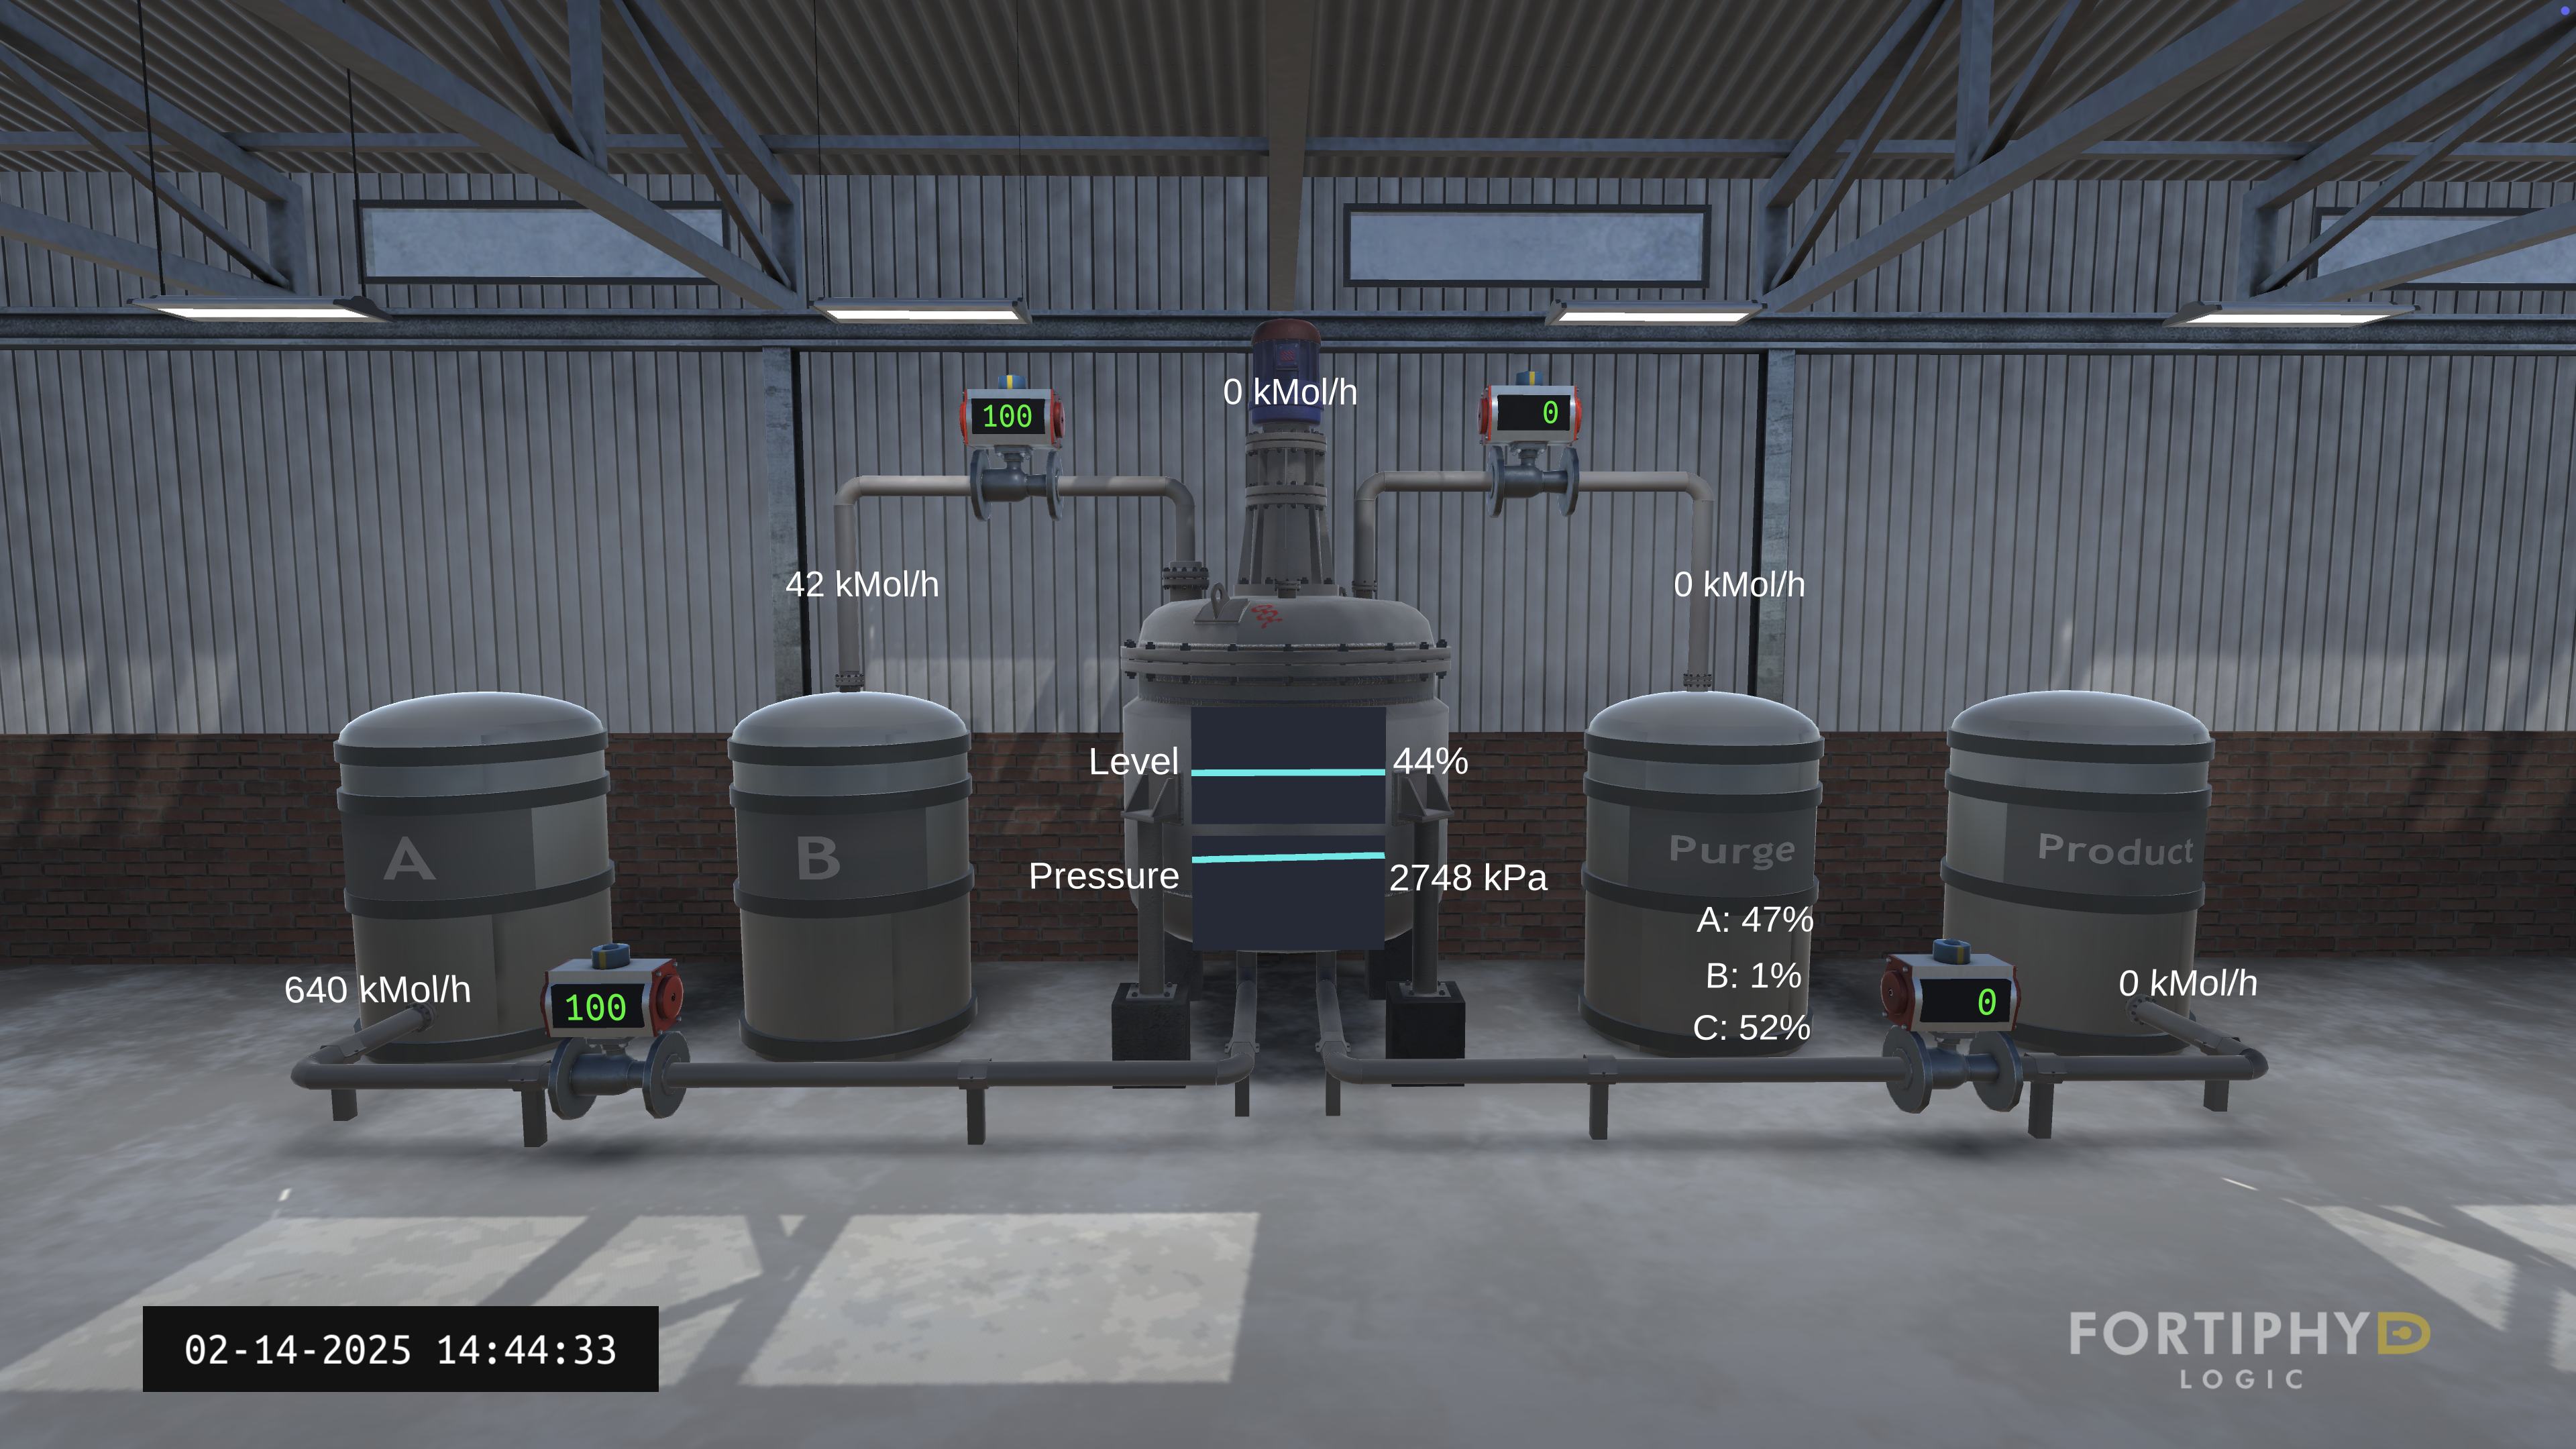
\includegraphics[keepaspectratio, width=0.6\linewidth]{Figures/Stage_1.png}
    \caption{GRFICS visualizer.}
    \label{fig:GRFICS}
\end{figure}
      valves and limited output measurements, this use case focuses on maintaining safe reactor pressure, optimizing chemical reaction efficiency, and minimizing waste. The controlled variables are two feed valves corresponding to the reactants (A and B), and the two output valves corresponding to the product (C) and purge tanks, respectively. The regulation of these valves at user-defined setpoints ensures system stability and safety, which is continuously monitored through sensor observations of pressure, liquid levels, and purge compositions. A Proportional-Derivative (PD) controller regulates the valve positions at user-defined setpoints through a master-slave Programmable Logic Controller (PLC).
    This emulation is hosted on a dedicated host machine within the OT network, labeled as the chemical plant in Figure \ref{fig:Chemical Plant}. The shaded squares within the chemical plant represent PLC slaves, which transmit sensor measurements to the master PLC for decision-making.

    \begin{figure}[!ht]
%     \vspace{-0.4cm}
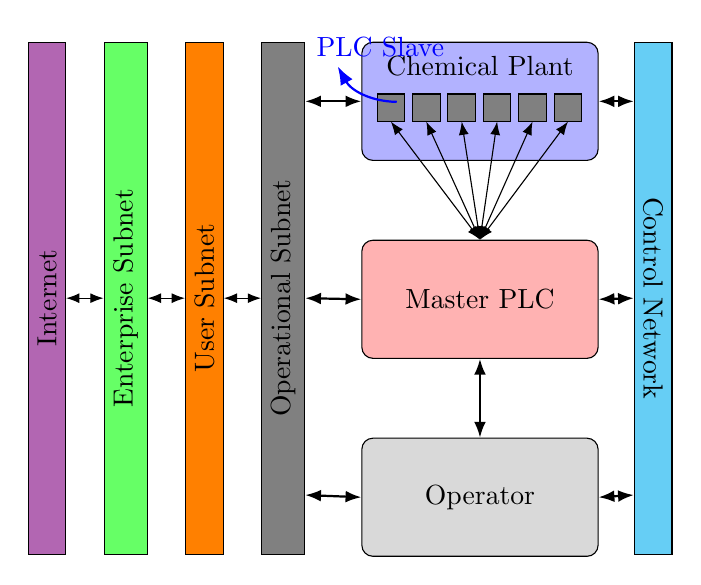
\begin{tikzpicture}
    \node[draw, rectangle, rounded corners, minimum width=3cm, minimum height=1.5cm, fill=blue!30, xshift=0cm] (rect1) {};
    \node[label={[yshift=0.075cm]north:Chemical Plant}] at (rect1.center) {};
    \foreach \x [count=\xi] in {1,...,6} {
        \coordinate (square-\xi) at ([xshift=-0.25cm + \x*0.45cm, yshift=0.5cm] rect1.south west);
        \draw (square-\xi) rectangle ++(0.35cm,0.35cm);
    }
    \foreach \x in {1,...,6} {
        \draw[fill=gray] ([xshift=-0.25cm + \x*0.45cm, yshift=0.5cm] rect1.south west) rectangle ++(0.35cm,0.35cm);
    }

    \node[draw, rectangle, rounded corners, minimum width=3cm, minimum height=1.5cm, fill=red!30, below=1cm of rect1] (rect2) {Master PLC};
    \node[draw, rectangle, rounded corners, minimum width=3cm, minimum height=1.5cm, fill=gray!30, below=1cm of rect2] (rect3) {Operator};
    \coordinate (top point) at ([xshift=4cm,yshift=0cm] rect1.north);
    \coordinate (bottom point) at ([xshift=4cm,yshift=0cm] rect3.south);
    % Adjusted distances to create gaps
\node[draw, rectangle, minimum width=6.5cm, minimum height=0.2cm, fill=cyan!60!white, rotate=270, right=-1.8cm of rect1.east] (controlrect) at ($(top point)!0!(bottom point)$) {{Control Network}};
\node[draw, rectangle, minimum width=6.5cm, minimum height=0.2cm, fill=violet!60!white, rotate=90, left=9.5cm of rect1.west] (publicrect) at ($(top point)!0!(bottom point)$) {{Internet}};
\node[draw, rectangle, minimum width=6.5cm, minimum height=0.2cm, fill=green!60!white, rotate=90, left=8.5cm of rect1.west] (enterrect) at ($(top point)!0!(bottom point)$) {{Enterprise Subnet}};
\node[draw, rectangle, minimum width=6.5cm, minimum height=0.2cm, fill=red!50!yellow, rotate=90, left=7.5cm of rect1.west] (userrect) at ($(top point)!0!(bottom point)$) {{User Subnet}};
\node[draw, rectangle, minimum width=6.5cm, minimum height=0.2cm, fill=black!50!white, rotate=90, left=6.5cm of rect1.west] (optrect) at ($(top point)!0!(bottom point)$) {{Operational Subnet}};

% The rest of the Ti*k*Z code remains the same...
    \foreach \x in {1,...,6} {
        \draw[Latex-Latex] (rect2.north) -- ($(square-\x.south)+(0.175,0cm)$);
    }
            \draw[thick, -Latex, blue] ([xshift=0.25cm, yshift=0.25cm]square-1) to[bend left] ([xshift=-0.5cm, yshift=0.7cm]square-1) node[anchor=south west,xshift=-0.4cm, blue] {PLC Slave};
    \draw[{Latex}-{Latex}] (publicrect.south) -- (enterrect.north);
    \draw[{Latex}-{Latex}] (enterrect.south) -- (userrect.north);
    \draw[{Latex}-{Latex}] (userrect.south) -- (optrect.north);
            
    \draw[thick, {Latex[length=2mm]}-{Latex[length=2mm]}] (rect1.east) -- ($(controlrect.south)+(0cm,2.5cm)$);
    \draw[thick, {Latex[length=2mm]}-{Latex[length=2mm]}] (rect2.east) -- ($(controlrect.south)+(0cm,0cm)$);
    \draw[thick, {Latex[length=2mm]}-{Latex[length=2mm]}] (rect3.east) -- ($(controlrect.south)+(0cm,-2.5cm)$);
    \draw[thick, {Latex[length=2mm]}-{Latex[length=2mm]}] (rect2.south) -- (rect3.north);
    \draw[thick, {Latex[length=2mm]}-{Latex[length=2mm]}] (rect1.west) -- ($(optrect.south)+(0cm,2.5cm)$);
    \draw[thick, {Latex[length=2mm]}-{Latex[length=2mm]}] (rect2.west) -- ($(optrect.south)+(0cm,0cm)$);
    \draw[thick, {Latex[length=2mm]}-{Latex[length=2mm]}] (rect3.west) -- ($(optrect.south)+(0cm,-2.5cm)$);
    
\end{tikzpicture}
% \vspace{-0.3cm}
    \caption{Chemical Plant workflow in Openstack.}
    \label{fig:Chemical Plant}
%     \vspace{-0.5cm}
\end{figure}
    \subsubsection{OpenPLC} It is an open-source PLC designed for ease of use, offering a cost-effective industrial automation solution suitable for both research and practical applications \cite{6970342}. It is compatible with a wide range of operating systems and, like traditional industrial PLCs, supports both discrete and continuous input interfaces through discrete input registers and coils, respectively. OpenPLC provides users with access to a limited set of registers, categorized as input, read and write registers, each named according to its specific function. The values stored in these registers can be utilized for informed decision-making, with controller logic programmed in standard PLC languages such as Structured Text (ST) and Ladder Diagram (LD). The PLC’s capacity can be expanded by connecting supported Modbus TCP devices, allowing additional slave PLCs to interface with the master PLC. Using Modbus, slave devices can read from and write to the master PLC’s registers via a standardized addressing system. This capability enables Modbus slaves to report sensor values to the master PLC by writing to its input registers and to execute controller decisions by reading from its holding registers. Modbus TCP utilizes TCP/IP for data exchange between devices such as PLCs and sensors, offering improved performance, scalability, and seamless integration with existing network infrastructures. Its reliability, even in harsh industrial environments, has made it a preferred choice for industrial communication.
    However, in Modbus TCP, packets are transmitted unencrypted to prioritize speed and efficiency, which makes the protocol susceptible to data falsification attacks and other cyber-threats, thereby limiting its use to industrial applications.
%    However, Modbus TCP is vulnerable to security risks, limiting its use to industrial applications. As packets are transmitted unencrypted, prioritizing speed and efficiency, the protocol is susceptible to data falsification attacks and other cyber threats. 
    
    \subsubsection{OpenPLC Client} It is a Python API that generates Modbus TCP API calls to interact with OpenPLC. Through its client interface, users can read and write the OpenPLC coils and registers. In our setup, the OpenPLC client runs on the operator node, where it reads and writes the OpenPLC registers and coils thereby
    % Additionally, the client can address both master and slave PLC devices, capturing and storing reported measurements in a database on the operator host for further analysis. 
    % By using the OpenPLC client for data monitoring and control, we
    bypassing the use of a dedicated Supervisory Control and Data Acquisition (SCADA) software like ScadaBR \cite{6938840}.
    
    













\balance
\section{Case Study}
\label{sec:casestudy}
This section describes the scenarios that demonstrate the use of the testbed proposed in this paper. In particular, we consider two scenarios separately to demonstrate the effect of network attacks. The adversarial attacks we demonstrate include Data Integrity Attacks (DIA) and Denial of Service Attacks (DoS). Table \ref{tab:attacks_comparison} highlights the key differences between the two attack types.
% \begin{itemize}
%     \item \textbf{Data Integrity Attacks (DIA) }are cyberattacks where an unauthorized party illicitly modifies the data stored, processed, or in transit within a system, thus compromising its accuracy and reliability. 
%     \item \textbf{Data Denial of Service Attacks (DoS)} target the availability of a service, intending to overwhelm the resources of a system, such as servers or networks, making it inaccessible to legitimate users
% \end{itemize}
% Table \ref{tab:attacks_comparison} summarizes the unique characteristics of the two attack types.
\begin{table}[!ht]
% \vspace{-0.3cm}
\centering
\caption{Attack comparison}
% \vspace{-0.3cm}
\label{tab:attacks_comparison}
\begin{tabular}{@{}>{\raggedright}p{0.2\linewidth}>{\raggedright\arraybackslash}p{0.35\linewidth}>{\raggedright\arraybackslash}p{0.35\linewidth}@{}}
\toprule
\textbf{Aspect} & \textbf{Data Integrity Attacks (DIA)} & \textbf{Denial of Service (DoS) Attacks} \\
\midrule
Primary Objective & Alter or corrupt data to undermine its accuracy and reliability. &  Make a network or service unavailable to its intended users. \\
% \addlinespace
% Impact on Services & Damages the correctness of information, leading to potential misuse. & Disrupts service availability, causing downtime and inaccessibility. \\
% \addlinespace
% Typical Methods & Malware, SQL injection, phishing, exploiting software vulnerabilities. & DoS attacks (distributed denial of service), SYN floods, ping of death, etc. \\
\addlinespace
Target & Data stored, in transit, or being processed. & Network infrastructure and servers. \\
\addlinespace
Detection & Requires monitoring for unauthorized data changes or anomalies. & Can often be detected by monitoring for sudden spikes in traffic. \\
% \addlinespace
% Goal of Attacker & To mislead, cause harm, or perpetrate fraud. & To disrupt operations, often for protest or to demand ransom. \\
\bottomrule
\end{tabular}
% \vspace{-0.6cm}
\end{table}

% We demonstrate the effect of these attacks on both the Power grid and Chemical Plant.

\subsection{Attacks on Power grid.}
The attacks on the Power Grid  include DoS and False Data Injection (FDI), which can be instigated at the communication path between any of the \textit{LC}s and the \textit{SC}. An adversary that succeeds in gaining control of the host machine becomes capable of manipulating the information transferred between the controllers or jamming the bandwidth to deny the information exchange between the controllers over the Mininet topology.  For demonstration purposes, we mimic the attacker behavior using a python script that will interfere with the functioning of each of these controllers. For DIA using FDI attack, we target the information being sent from the controllers (\textit{SC} or \textit{LC}) and manipulate it by running a script in parallel that will replace this data while ensuring higher priority/rank for the substation.
\begin{figure}[!ht]
% \vspace{-0.2cm}
    \centering
    
\includegraphics[width=\linewidth]{Figures/legend_only.pdf} \\
%     \vspace{-0.1cm}
    \definecolor{dark_contrast}{HTML}{006400}
    \def\linenda{0.987}
    \def\linendb{0.987}
    \begin{tikzpicture}
        \node[anchor=south west,inner sep=0] (image) at (0,0) {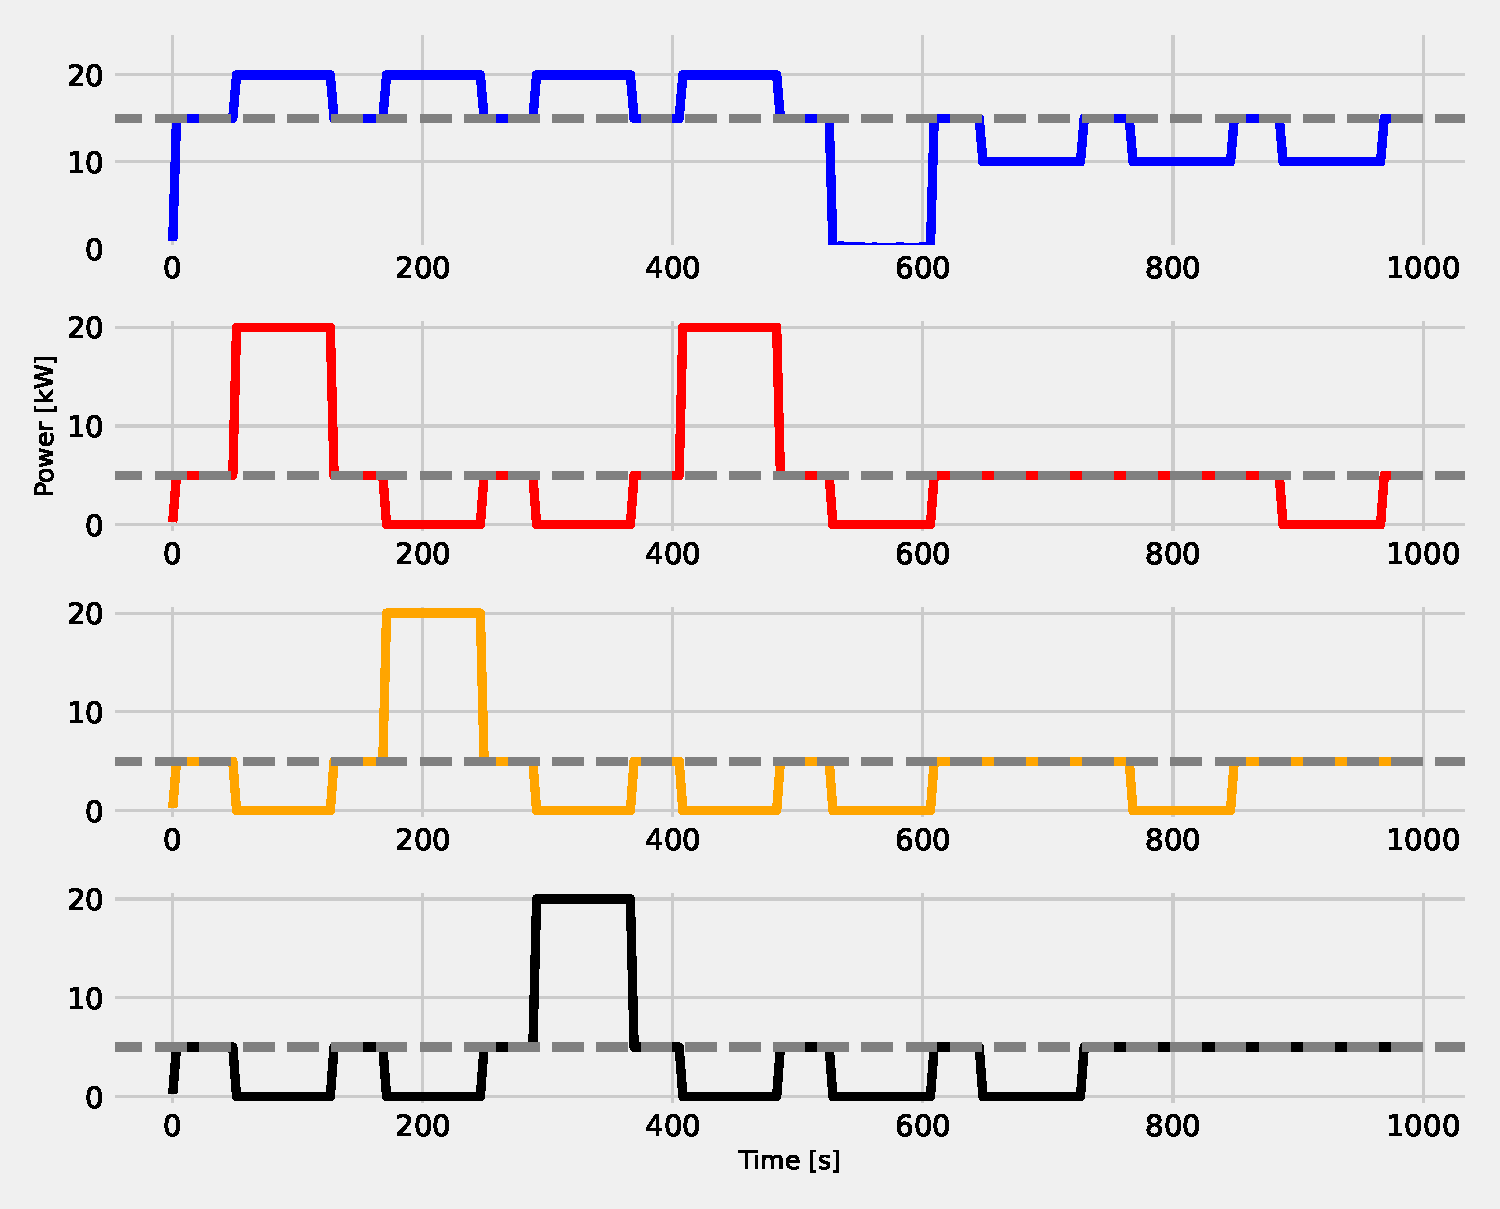
\includegraphics[width=\linewidth]{Figures/demand_and_supply.pdf}};
        \begin{scope}[x={(image.south east)},y={(image.north west)}]
            \draw [dark_contrast, thick, dashed, line width=0.75pt] (0.156,0) -- (0.156,\linenda) node [above, black] {};
            \draw [dark_contrast, thick, dashed, line width=0.75pt] (0.222,0) -- (0.222,\linenda);
            \node[red, text width=3cm, align=center] at (0.19,1) {\tiny{FDI-$lc_1$}};
            
            \draw [dark_contrast, thick, dashed, line width=0.75pt] (0.256,0) -- (0.256,\linendb) node [above, black] {};
            \draw [dark_contrast, thick, dashed, line width=0.75pt] (0.322,0) -- (0.322,\linendb);
            \node[red, text width=3cm, align=center] at (0.29,1) {\tiny{FDI-$lc_2$}};

            \draw [dark_contrast, thick, dashed, line width=0.75pt] (0.356,0) -- (0.356,\linenda) node [above, black] {};
            \draw [dark_contrast, thick, dashed, line width=0.75pt] (0.422,0) -- (0.422,\linenda);
            \node[red, text width=3cm, align=center] at (0.39,1) {\tiny{FDI-$lc_3$}};

            \draw [dark_contrast, thick, dashed, line width=0.75pt] (0.456,0) -- (0.456,\linendb) node [above, black] {};
            \draw [dark_contrast, thick, dashed, line width=0.75pt] (0.522,0) -- (0.522,\linendb);
            \node[red, text width=3cm, align=center] at (0.49,1) {\tiny{FDI-$sc$}};

            \draw [dark_contrast, thick, dashed, line width=0.75pt] (0.556,0) -- (0.556,\linenda) node [above, black] {};
            \draw [dark_contrast, thick, dashed, line width=0.75pt] (0.622,0) -- (0.622,\linenda);
            \node[red, text width=3cm, align=center] at (0.59,1) {\tiny{DoS-$sc$}};

            \draw [dark_contrast, thick, dashed, line width=0.75pt] (0.656,0) -- (0.656,\linendb) node [above, black] {};
            \draw [dark_contrast, thick, dashed, line width=0.75pt] (0.722,0) -- (0.722,\linendb);
            \node[red, text width=3cm, align=center] at (0.69,1) {\tiny{DoS-$lc_3$}};

            \draw [dark_contrast, thick, dashed, line width=0.75pt] (0.756,0) -- (0.756,\linenda) node [above, black] {};
            \draw [dark_contrast, thick, dashed, line width=0.75pt] (0.822,0) -- (0.822,\linenda);
            \node[red, text width=3cm, align=center] at (0.79,1) {\tiny{DoS-$lc_2$}};        

            \draw [dark_contrast, thick, dashed, line width=0.75pt] (0.856,0) -- (0.856,\linendb) node [above, black] {};
            \draw [dark_contrast, thick, dashed, line width=0.75pt] (0.922,0) -- (0.922,\linendb);
            \node[red, text width=3cm, align=center] at (0.89,1) {\tiny{DoS-$lc_1$}};
        % \draw [rounded corners, thick] (0.05,-0.03) rectangle (0.95,0.01);
        %     \node at (0.5,-0.015) {\tiny{FDI: False Data Injection, DoS: Denial of Service, $lc_{i}$: local controller $i$, sc: supervisory controller}};    
        \end{scope}
    \end{tikzpicture}
%     \vspace{-0.5cm}
    \caption{Visualization of demand and supply values under attacks. FDI and DoS correspond to the False Data Injection and Denial of Service respectively, while $lc_i$ and $sc$ depicts  the attacked local and supervisory controllers respectively. }
    \label{fig:grid_attack}
%     \vspace{-0.1cm}
\end{figure}
  For instance, if the local controller associated with substation 1, \textit{LC}1, demands a higher power beyond the power grid capacity (20kW) at the highest priority, then \textit{LC}2 and \textit{LC}3 (requesting a steady 5kW for the next sampling interval) are forced to send their respective substations to island mode. Figure \ref{fig:grid_attack} shows the demand and supply of the \textit{SC} and \textit{LC}s under the FDI attacks on each of the controllers. 
  The first four annotations in the Figure correspond to FDI attacks on \textit{LC}1, \textit{LC}2, \textit{LC}3, and the \textit{SC} respectively. 

To replicate a DoS attack, a Python script running in parallel threads disrupts communication between Local Controllers and the Supervisory Controller. This interruption prevents information from reaching its intended destination, effectively blocking updates. As a result, in the absence of communication, the system interprets the missing data as 0 kW demand (from an \textit{LC}) or 0 kW supply (from the \textit{SC}), causing the affected substation to enter islanding mode. The impact of this attack is visualized through plots in Figure \ref{fig:grid_attack} where
the last four annotations illustrate DoS attacks targeting the \textit{SC}, \textit{LC}3, \textit{LC}2, and \textit{LC}1, respectively. 

Each attack type exhibits a distinct supply-demand pattern, which can be compared against the actual demand and supply values recorded at the GridLAB-D logs. This comparison is the key observation for attack detection and type.The current stage of this test bed features only one actuator (a load switch for islanding) for power regulation. We manually regulate the load module within GridLAB-D to adjust the load value and maintain a constant voltage for the power supplied. In the future, this will be improved by adding more ZIP loads connected to the substation, equipped with custom switches that can modify the overall load. This enhancement will provide more granular observations beyond the discrete levels depicted in Figure \ref{fig:grid_attack}.



% \begin{figure}[H]
%     % First row
%     \begin{subfigure}{0.5\linewidth}
%         \hspace*{-1.5cm} % Adjust the value as needed to shift the image to the left
%         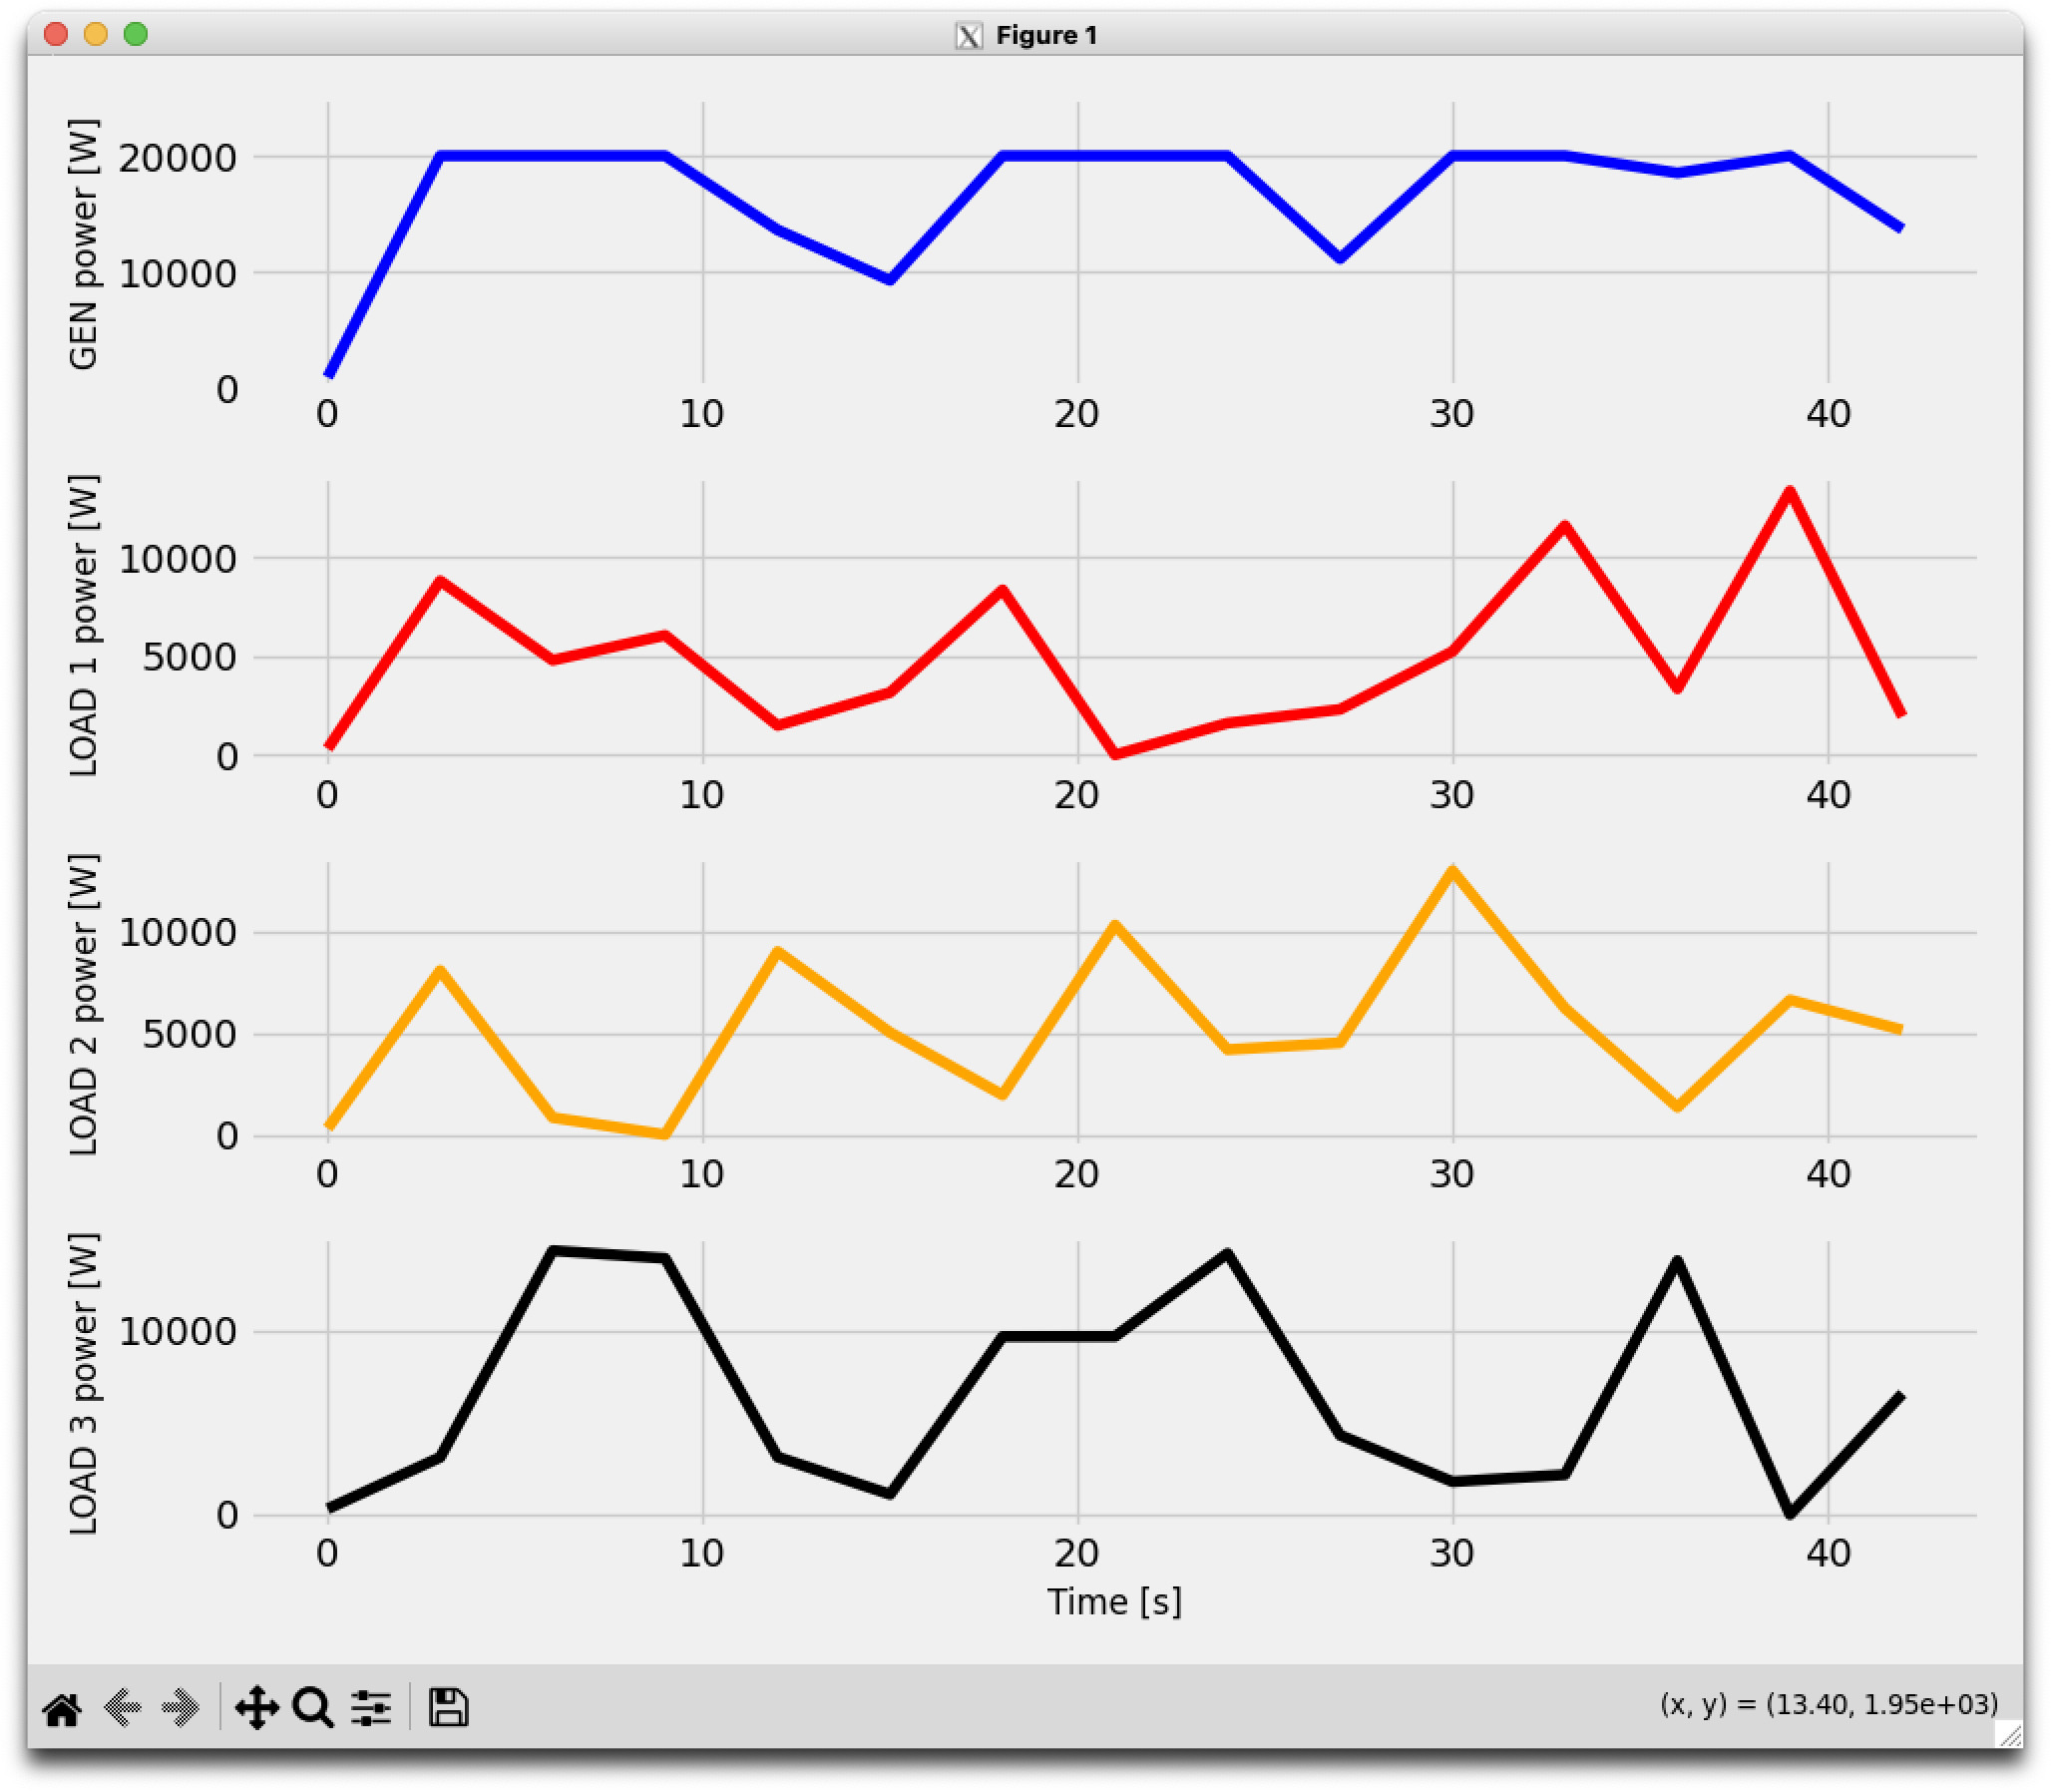
\includegraphics[width=8cm,keepaspectratio]{Figures/normal_mode.png}
%         \caption{}
%         \label{fig:no_attack}
%     \end{subfigure}
%     % You may remove the vspace if you don't need extra vertical space between the subfigures
%     \vspace{1cm} 
%     \begin{subfigure}{0.5\linewidth}
%         \hspace*{-1.5cm} % Adjust the value as needed to shift the image to the left
%         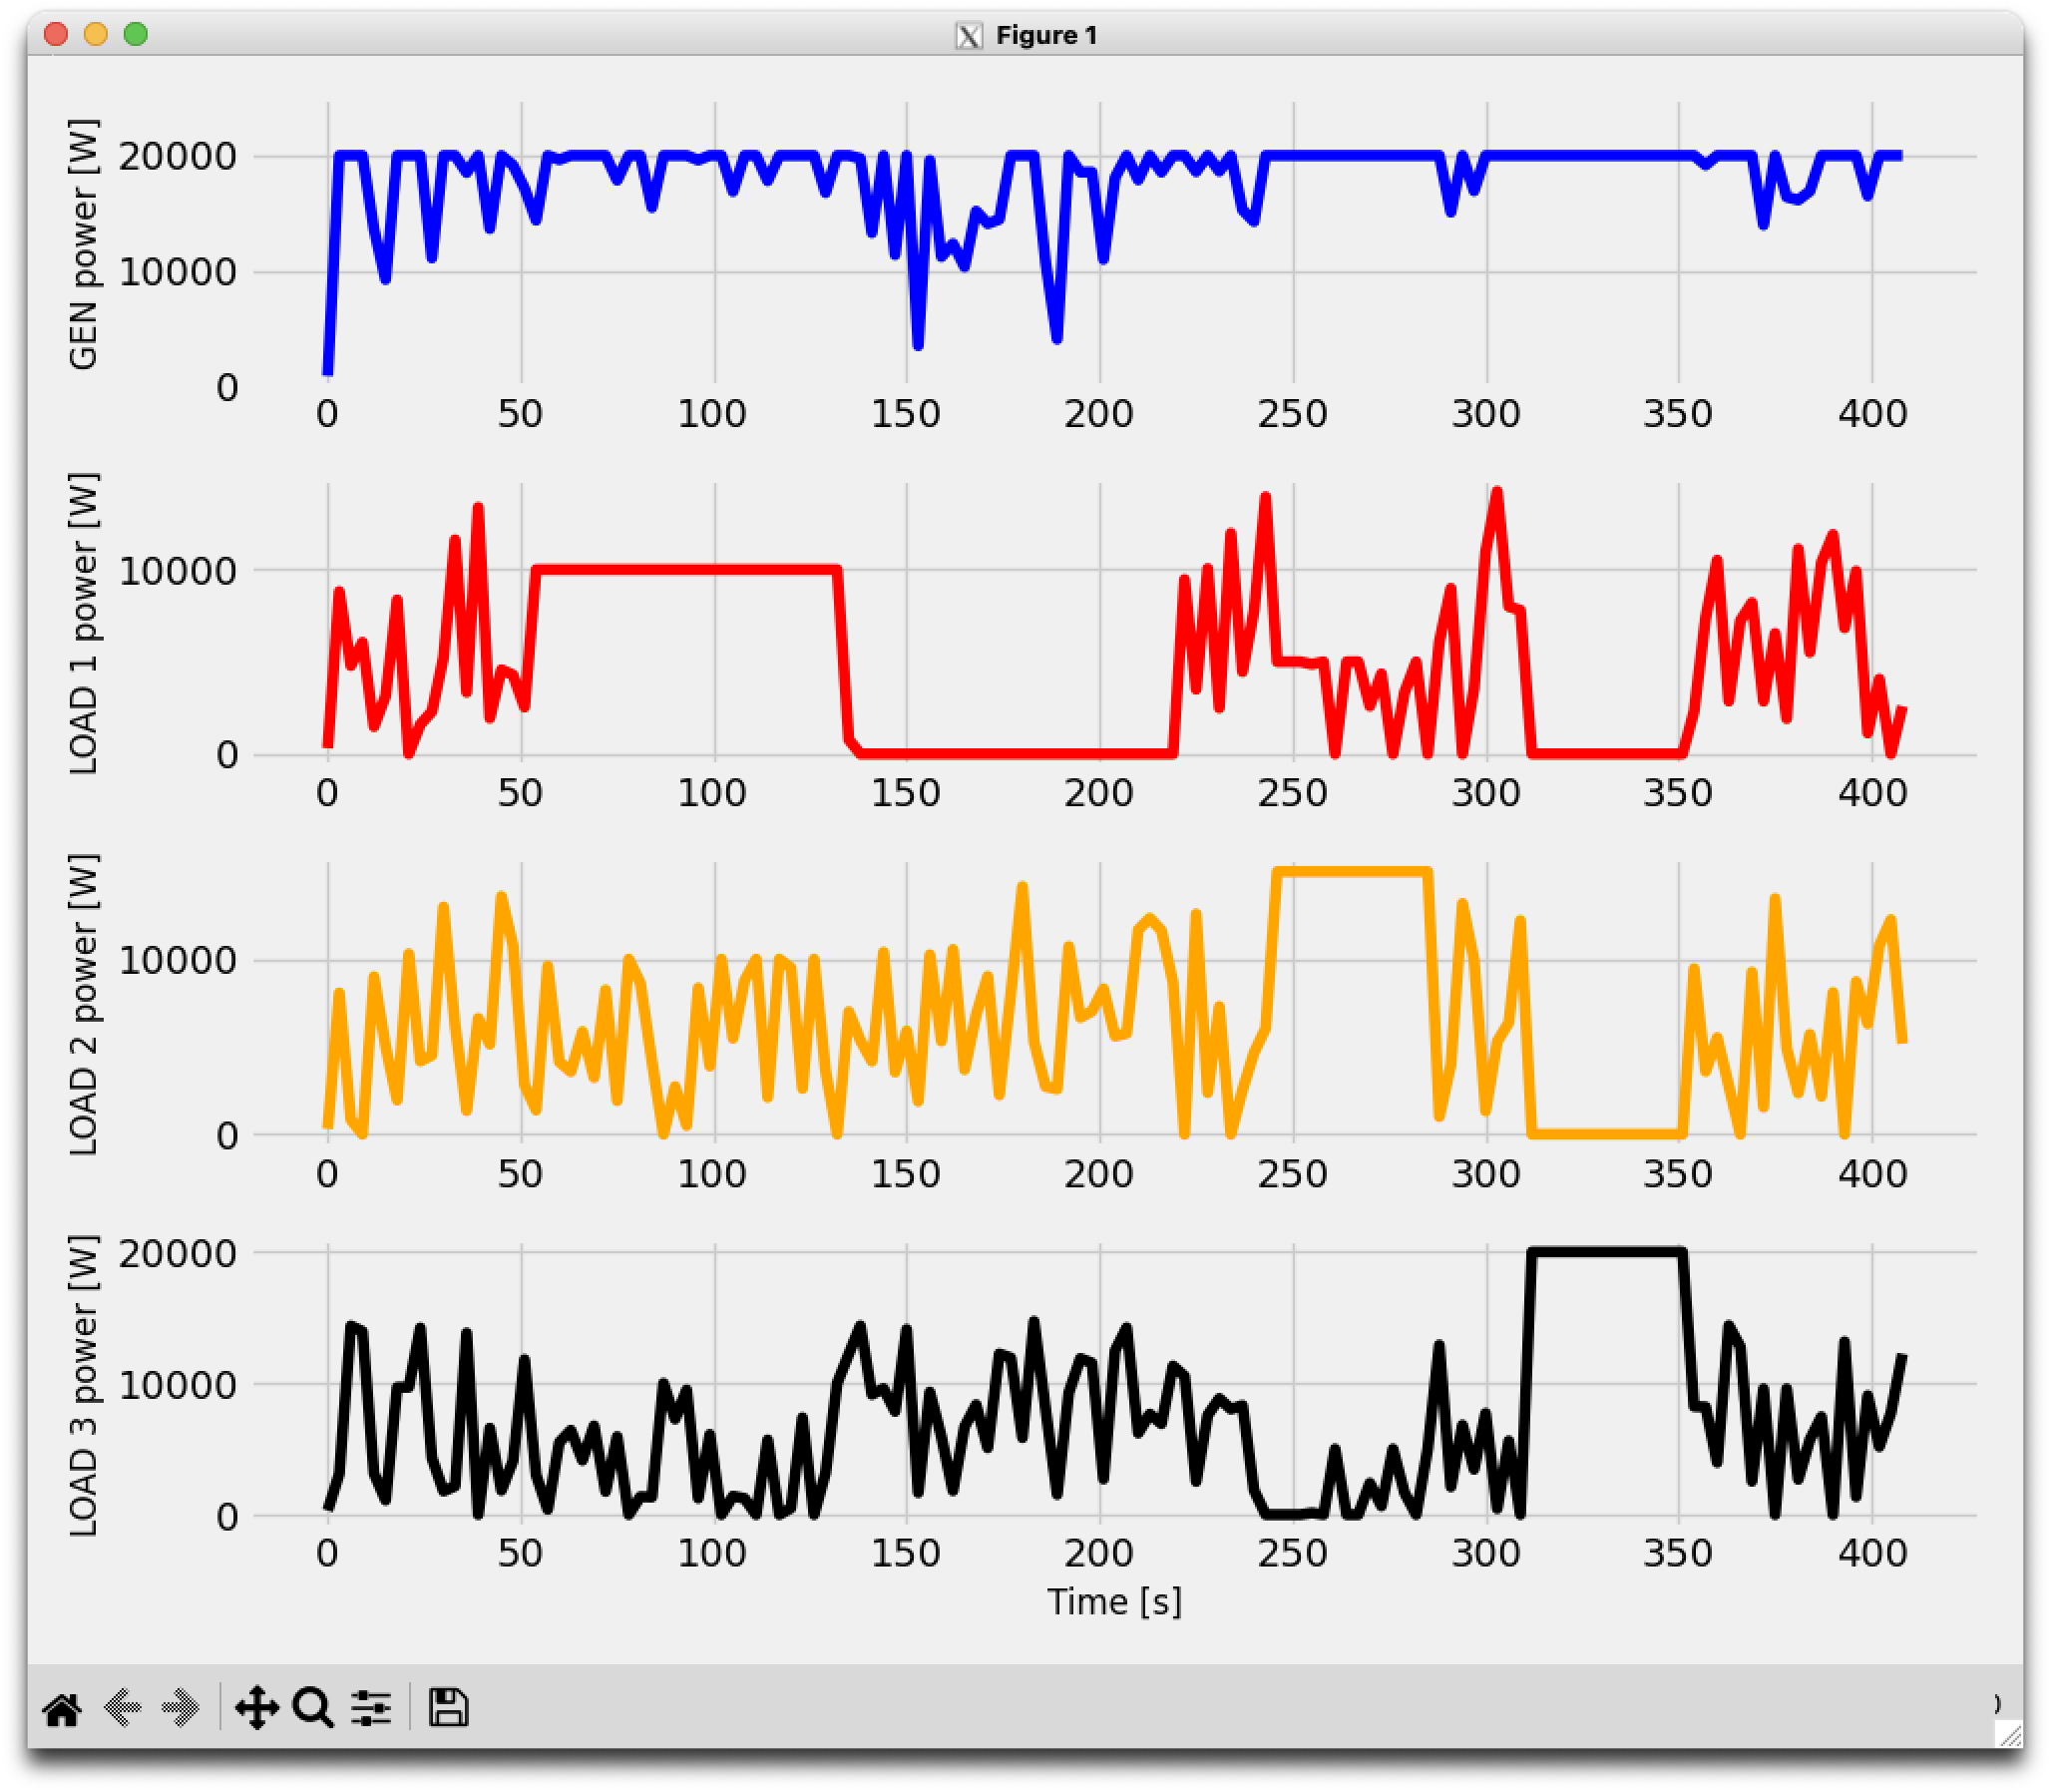
\includegraphics[width=8cm,keepaspectratio]{Figures/different_attacks.png}
%         \caption{}
%         \label{fig:with_attack}
%     \end{subfigure}
%     \caption{Different stages in the power grid attack resulting in islanding.}
%     \label{fig:grid_attack}
% \end{figure}


% \begin{figure}
%         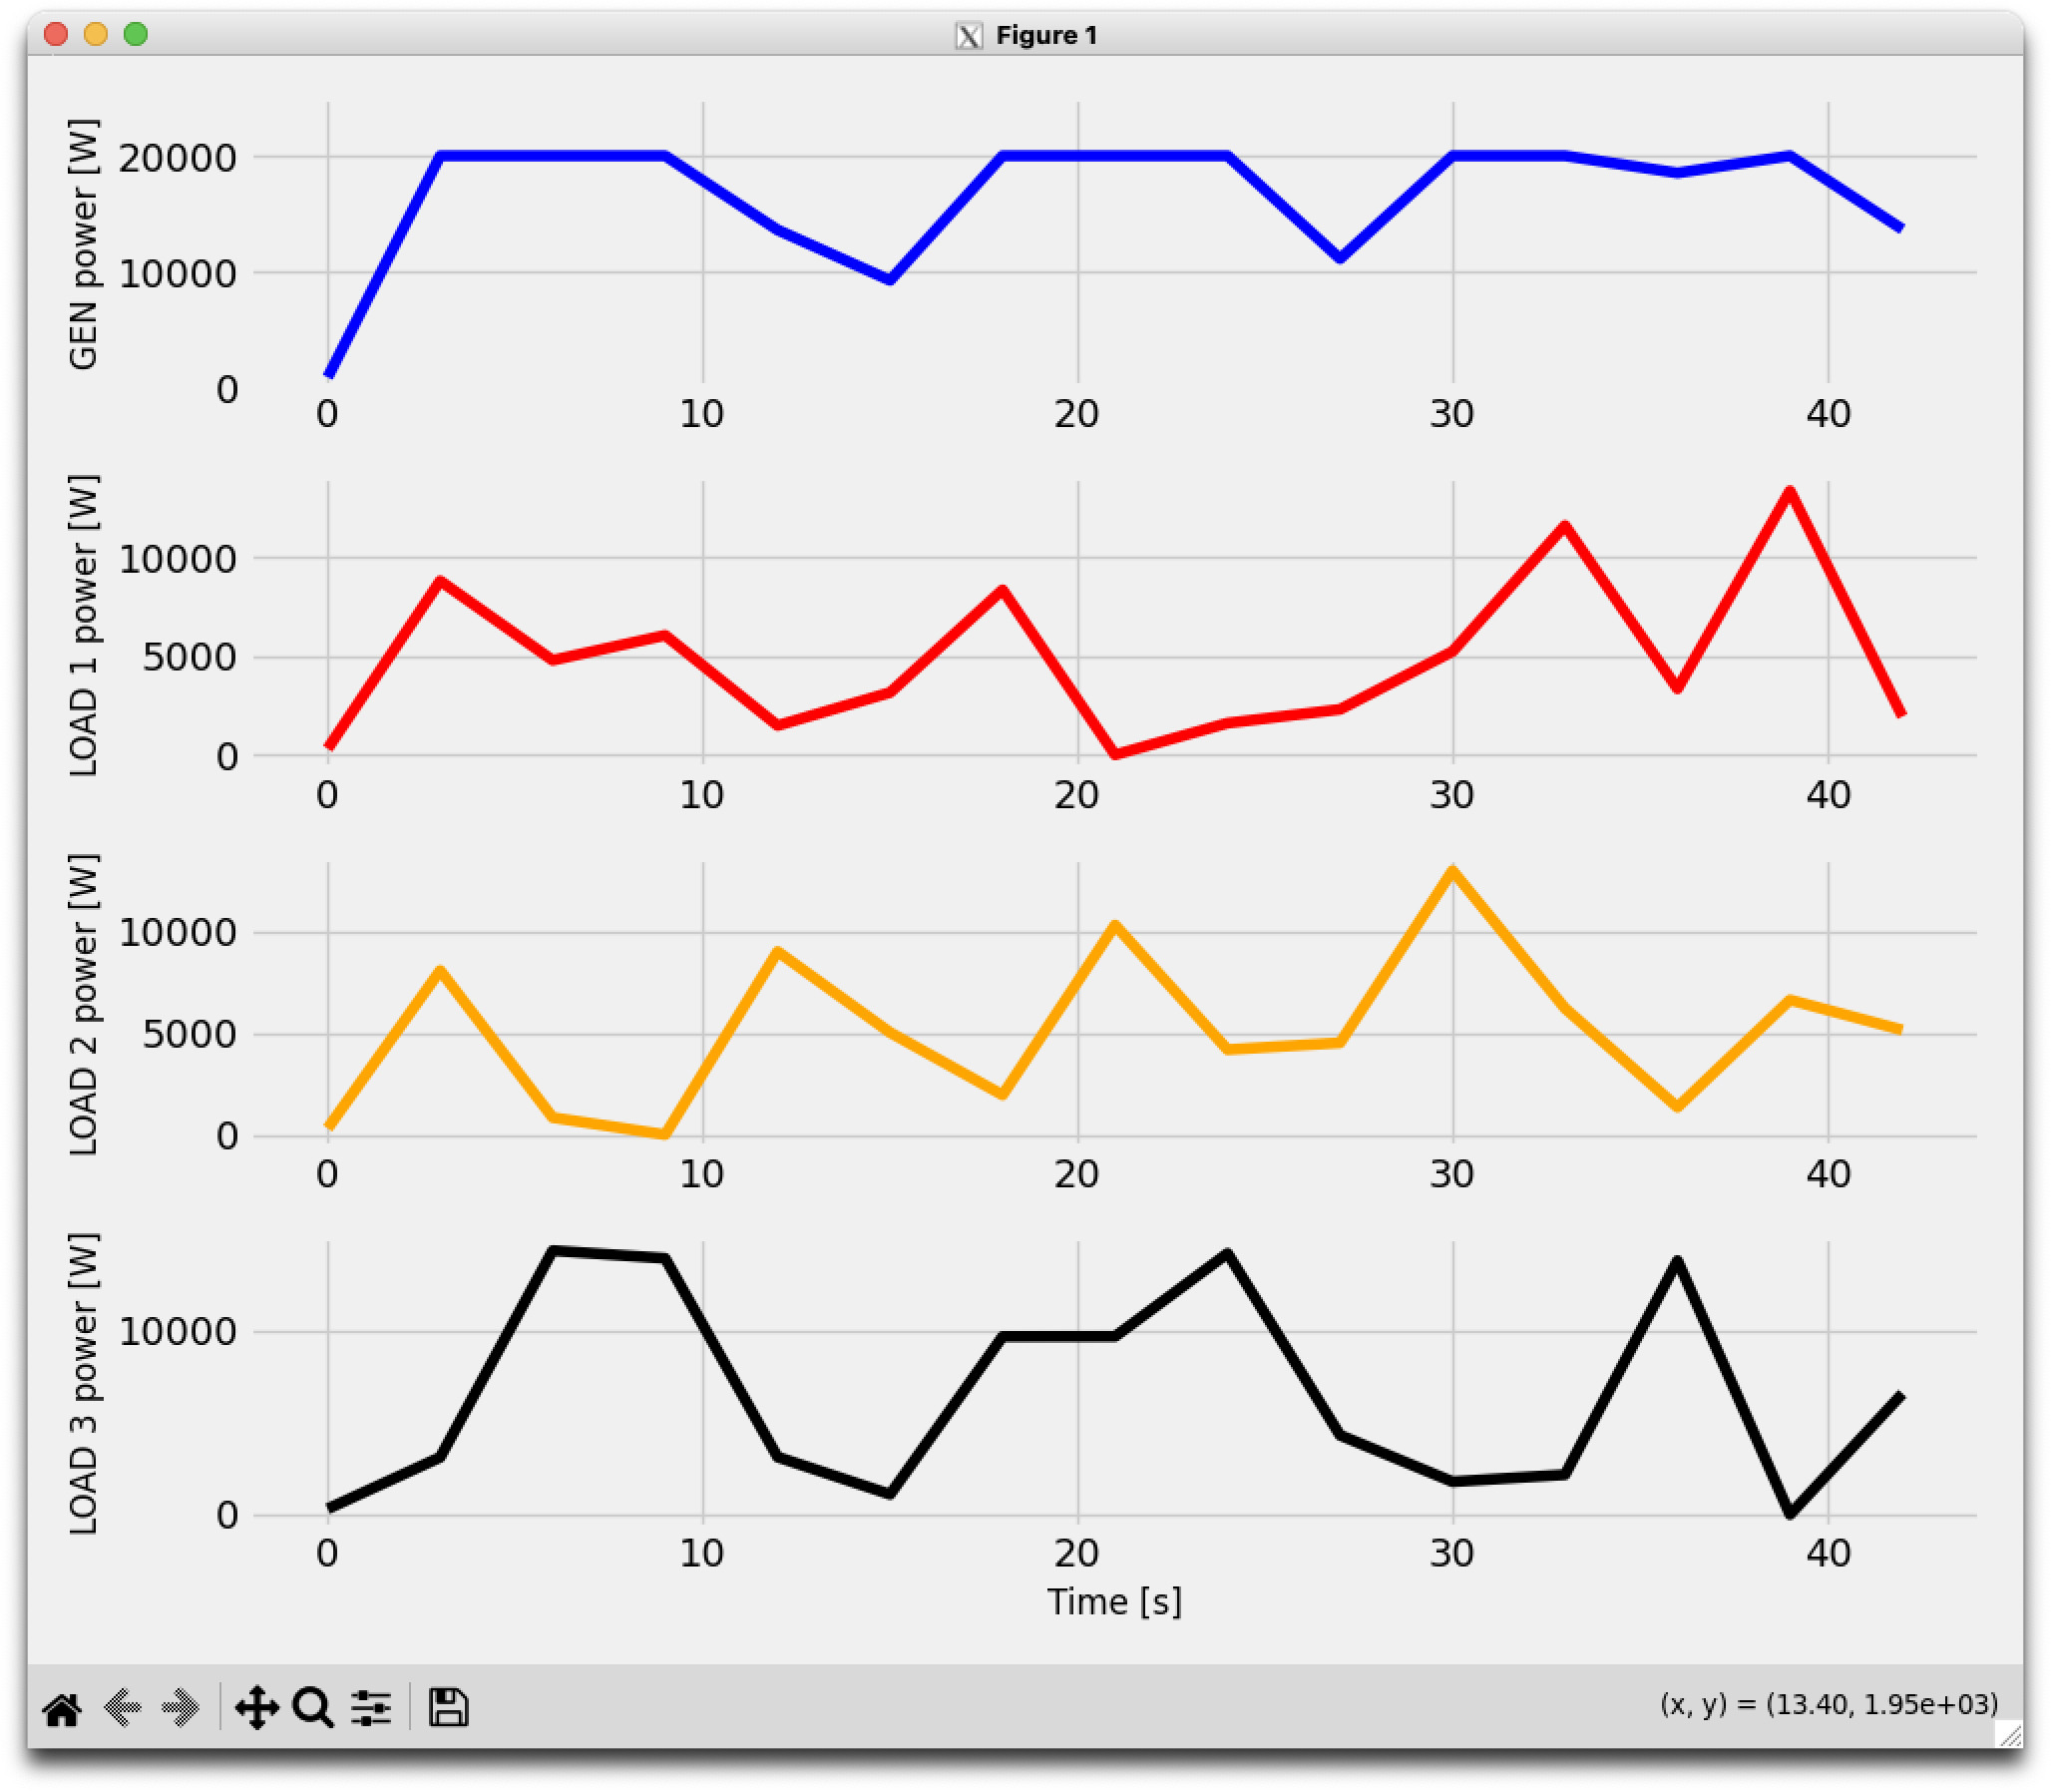
\includegraphics[width=8cm,keepaspectratio]{Figures/normal_mode.png}
%         \caption{}
%         \label{fig:no_attack}
% \end{figure}




\subsection{Attacks on Chemical Plant}
% \begin{figure}[H]
% \begin{tikzpicture}
%     \node[draw, rectangle, rounded corners, minimum width=3.5cm, minimum height=1.5cm, fill=blue!30] (rect1) {};
%     \node[label={[yshift=0.2cm]north:Chemical Plant}] at (rect1.center) {};
    
%     \foreach \x [count=\xi] in {1,...,6} {
%         \coordinate (square-\xi) at ([xshift=-0.2cm + \x*0.5cm, yshift=0.5cm] rect1.south west);
%         \draw (square-\xi) rectangle ++(0.4cm,0.4cm);
%     }
%     \foreach \x in {1,...,6} {
%         \draw[fill=gray] ([xshift=-0.2cm + \x*0.5cm, yshift=0.5cm] rect1.south west) rectangle ++(0.4cm,0.4cm);
%     }
%         \draw[thick, dotted, -Latex] ([xshift=0.25cm, yshift=0.25cm]square-1) to[bend left] ([xshift=-1cm, yshift=1cm]square-1) node[anchor=south west, fill=white] {Sensor};


%     \node[draw, rectangle, rounded corners, minimum width=3.5cm, minimum height=1.5cm, fill=red!30, below=1cm of rect1] (rect2) {Master PLC};
%     \coordinate (top point) at ([xshift=4cm,yshift=0cm] rect1.north);
%     \coordinate (bottom point) at ([xshift=4cm,yshift=0cm] rect2.south);

%     \node[draw, rectangle, minimum width=4cm, minimum height=0.5cm, fill=green!30, rotate=270, right=1cm of rect1.east |-
%     rect2.east] (longrect) at ($(top point)!0!(bottom point)$) {Control Network};



% \foreach \x in {1,...,6} {
%     \ifodd\x\relax
%         \draw[Latex-Latex] (rect2.north) -- ($(square-\x.south)+(0.2,0cm)$);
%     \else
%         \draw[thick, dotted, Latex-Latex] (rect2.north) -- ($(square-\x.south)+(0.2,0cm)$);
%     \fi
% }
%     \draw[thick, {Latex[length=2mm]}-{Latex[length=2mm]}] (rect1.east) -- ($(longrect.south)+(0cm,1.25cm)$);
%     \draw[thick, {Latex[length=2mm]}-{Latex[length=2mm]}] (rect2.east) -- ($(longrect.south)+(0cm,-1.25cm)$);
% \end{tikzpicture}
%     \caption{Schematic depicting the chemical plant under availability attacks. The dotted arrows between the plant and plc are the sensor information blocked as a consequence of the attack.}
%     \label{fig:Chemical_DoS}
%     \Description{DoS chemical plant attack}
% \end{figure}
Figure \ref{fig:Chemical_attacks} shows the schematic of the attack implementations on the Chemical Plant. An attacker gaining access to the hosts can initiate these attacks by intercepting the information sent and received between the PLC and the plant.   
% \begin{figure}
%     \centering
%     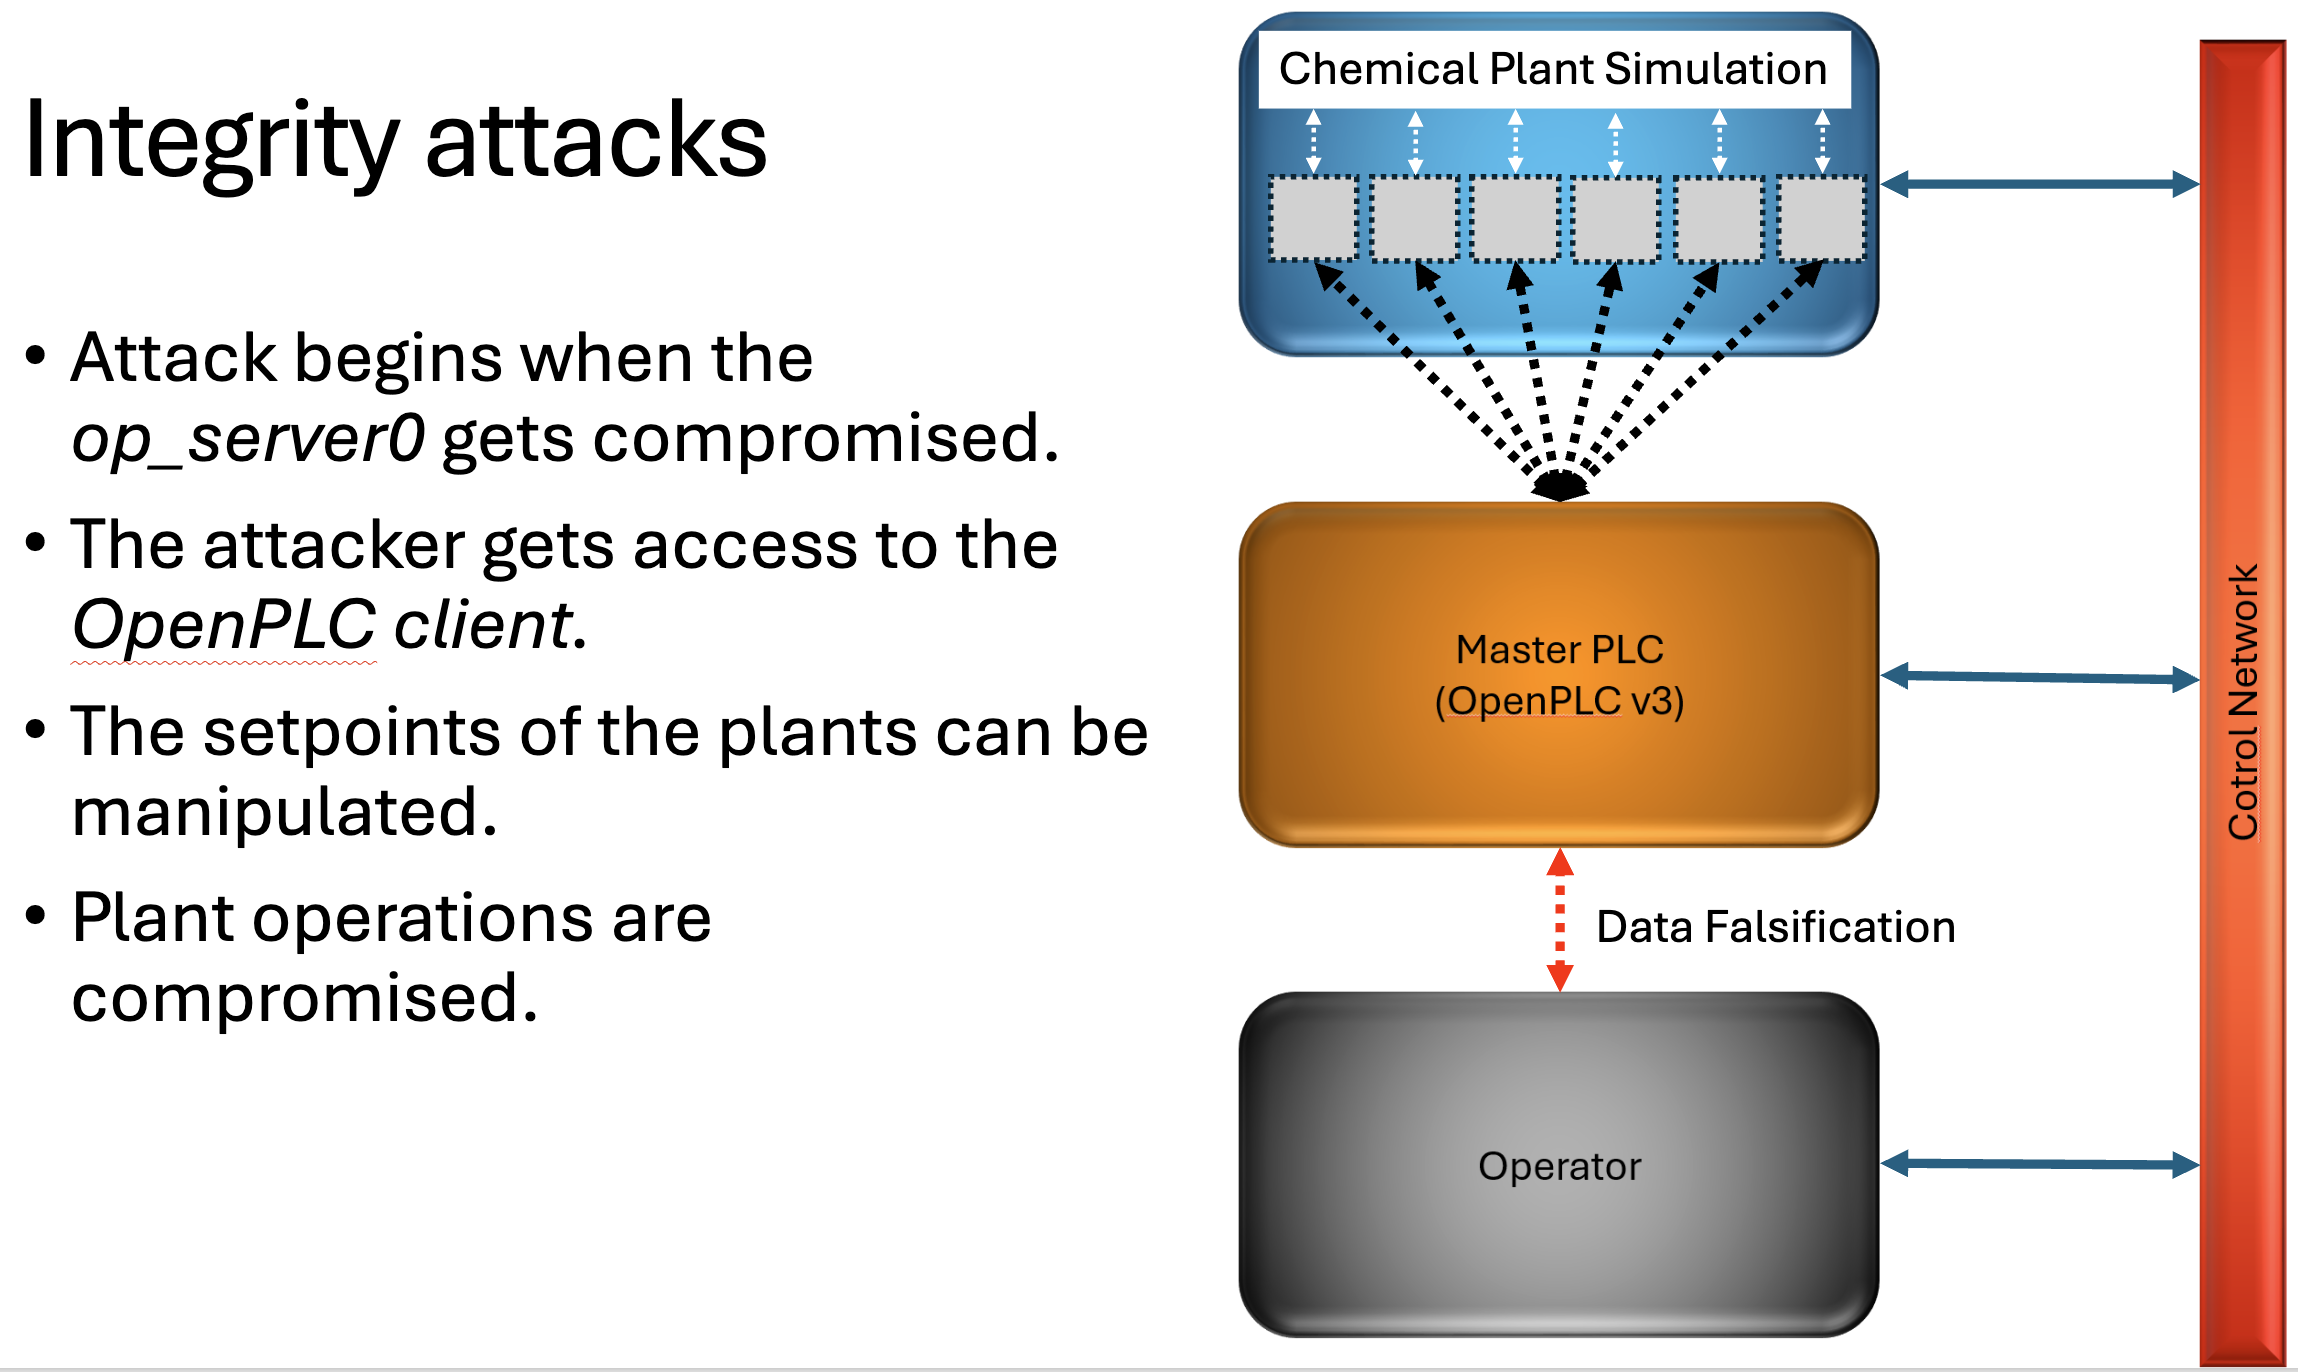
\includegraphics[width=\linewidth]{Figures/ChemicalPlantIntegrity.png}
%     \caption{Schematic showing the chemical plant under integrity attacks.}
%     \label{fig:Chemical_DIA}
% \end{figure}
\begin{figure}[!htbp]
\centering
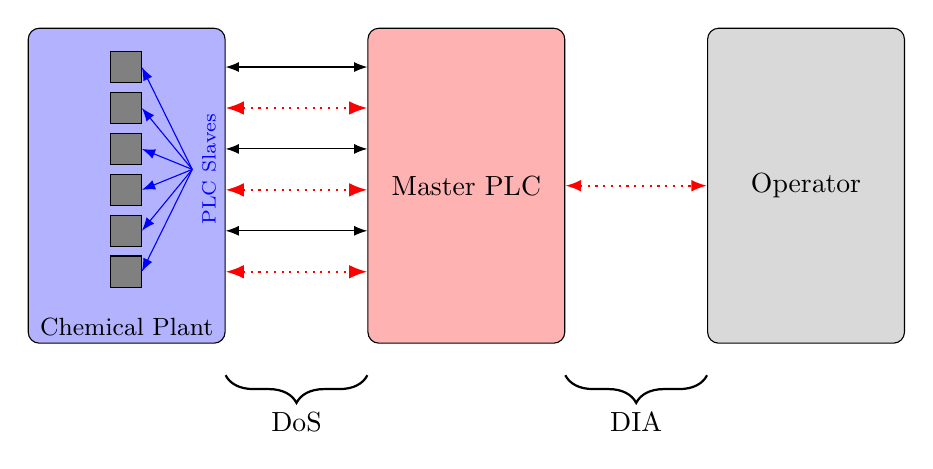
\begin{tikzpicture}[decoration={brace,amplitude=10pt}]
    % Chemical Plant (left): tall box, "Chemical Plant" horizontal at bottom
    \node[draw, rectangle, rounded corners, minimum width=2.5cm, minimum height=4.0cm, fill=blue!30] (rect1) {};
    \node[font=\small] at ([yshift=0.22cm] rect1.south) {Chemical Plant};

    % PLC slave squares: sq-\y = bottom-left, sqc-\y = centre of each square
    \foreach \y in {1,...,6} {
        \coordinate (sq-\y)  at ([xshift=1.05cm, yshift={-0.7cm - (\y-1)*0.52cm}] rect1.north west);
        \coordinate (sqc-\y) at ([xshift=1.25cm, yshift={-0.5cm - (\y-1)*0.52cm}] rect1.north west);
        \draw[fill=gray] (sq-\y) rectangle ++(0.4cm, 0.4cm);
    }

    % "PLC Slaves" label: rotated 90 deg, aligned on right edge of rect1
    \node[rotate=90, font=\scriptsize, color=blue] (plclabel)
        at ([xshift=2.3cm, yshift={-0.5cm - 2.5*0.52cm}] rect1.north west) {PLC Slaves};

    % 6 arrows fanning from centre of PLC Slaves label to each square
    \foreach \y in {1,...,6} {
        \draw[-Latex, thin, color=blue]
            (plclabel.north)
            -- ($(sq-\y) + (0.4cm, 0.2cm)$);
    }

    % Master PLC (centre)
    \node[draw, rectangle, rounded corners, minimum width=2.5cm, minimum height=4.0cm,
          fill=red!30, right=1.8cm of rect1] (rect2) {Master PLC};

    % Operator (right)
    \node[draw, rectangle, rounded corners, minimum width=2.5cm, minimum height=4.0cm,
          fill=gray!30, right=1.8cm of rect2] (rect3) {Operator};

    % Horizontal data-flow arrows: Chemical Plant to Master PLC
    % Odd = solid black (normal);  Even = dotted red (compromised)
    \foreach \y in {1,...,6} {
        \ifodd\y\relax
            \draw[Latex-Latex] (rect1.east |- sqc-\y) -- (rect2.west |- sqc-\y);
        \else
            \draw[thick, dotted, Latex-Latex, color=red] (rect1.east |- sqc-\y) -- (rect2.west |- sqc-\y);
        \fi
    }

    % DIA arrow: Master PLC to Operator (horizontal, dotted red)
    \draw[thick, dotted, {Latex[length=2mm]}-{Latex[length=2mm]}, color=red]
        (rect2.east) -- (rect3.west);

    % DoS brace: width of the rect1-rect2 gap only, arch pointing downward
    \draw[decorate, decoration={brace, mirror}, thick]
        ([yshift=-0.4cm] rect1.south east) -- ([yshift=-0.4cm] rect2.south west)
        node[midway, yshift=-0.6cm] {DoS};

    % DIA brace: width of the rect2-rect3 gap only, arch pointing downward
    \draw[decorate, decoration={brace, mirror}, thick]
        ([yshift=-0.4cm] rect2.south east) -- ([yshift=-0.4cm] rect3.south west)
        node[midway, yshift=-0.6cm] {DIA};
\end{tikzpicture}
    \caption{Schematic showing the chemical plant under integrity attacks. The dotted red arrow represents the information corrupted by the attack.}
    \label{fig:Chemical_attacks}
%     \vspace{-0.2cm}
\end{figure}
In DIA, the setpoints inside the PLC registers for regulating the valves of the chemical plants are manipulated. This can lead to instability of the chemical plant and if not prevented can lead to explosion. 
Similarly, in a DoS attack scenario, the attacker jams the communication spectrum between the controller and the plant with random noise, disrupting data transmission. Such interference in the critical communication channel can be highly dangerous, potentially leading to system instability and, in extreme cases, triggering an explosion. 

This paper focuses on demonstrating the effect of an attack and the provisioning available within the host machines for the users to detect a potential threat. Therefore, we mimic an attack type that faithfully replicates its effect compared to its real-world implementation. For example we forcefully manipulate the data in the PLC registers, with the assumption that the attacker has gained access to the operational server. Similarly, rather than jamming the network in case of a DoS attack, we manually stop the sensor information from reaching its destination. 
% We instigate the DoS action using the python scripts that can stop the chosen services on the chemical plant host that deals with the Modbus slaves.

\begin{figure}[!htbp]
% \vspace{-0.2cm}
    \centering
    \begin{subfigure}{0.49\linewidth}
        \centering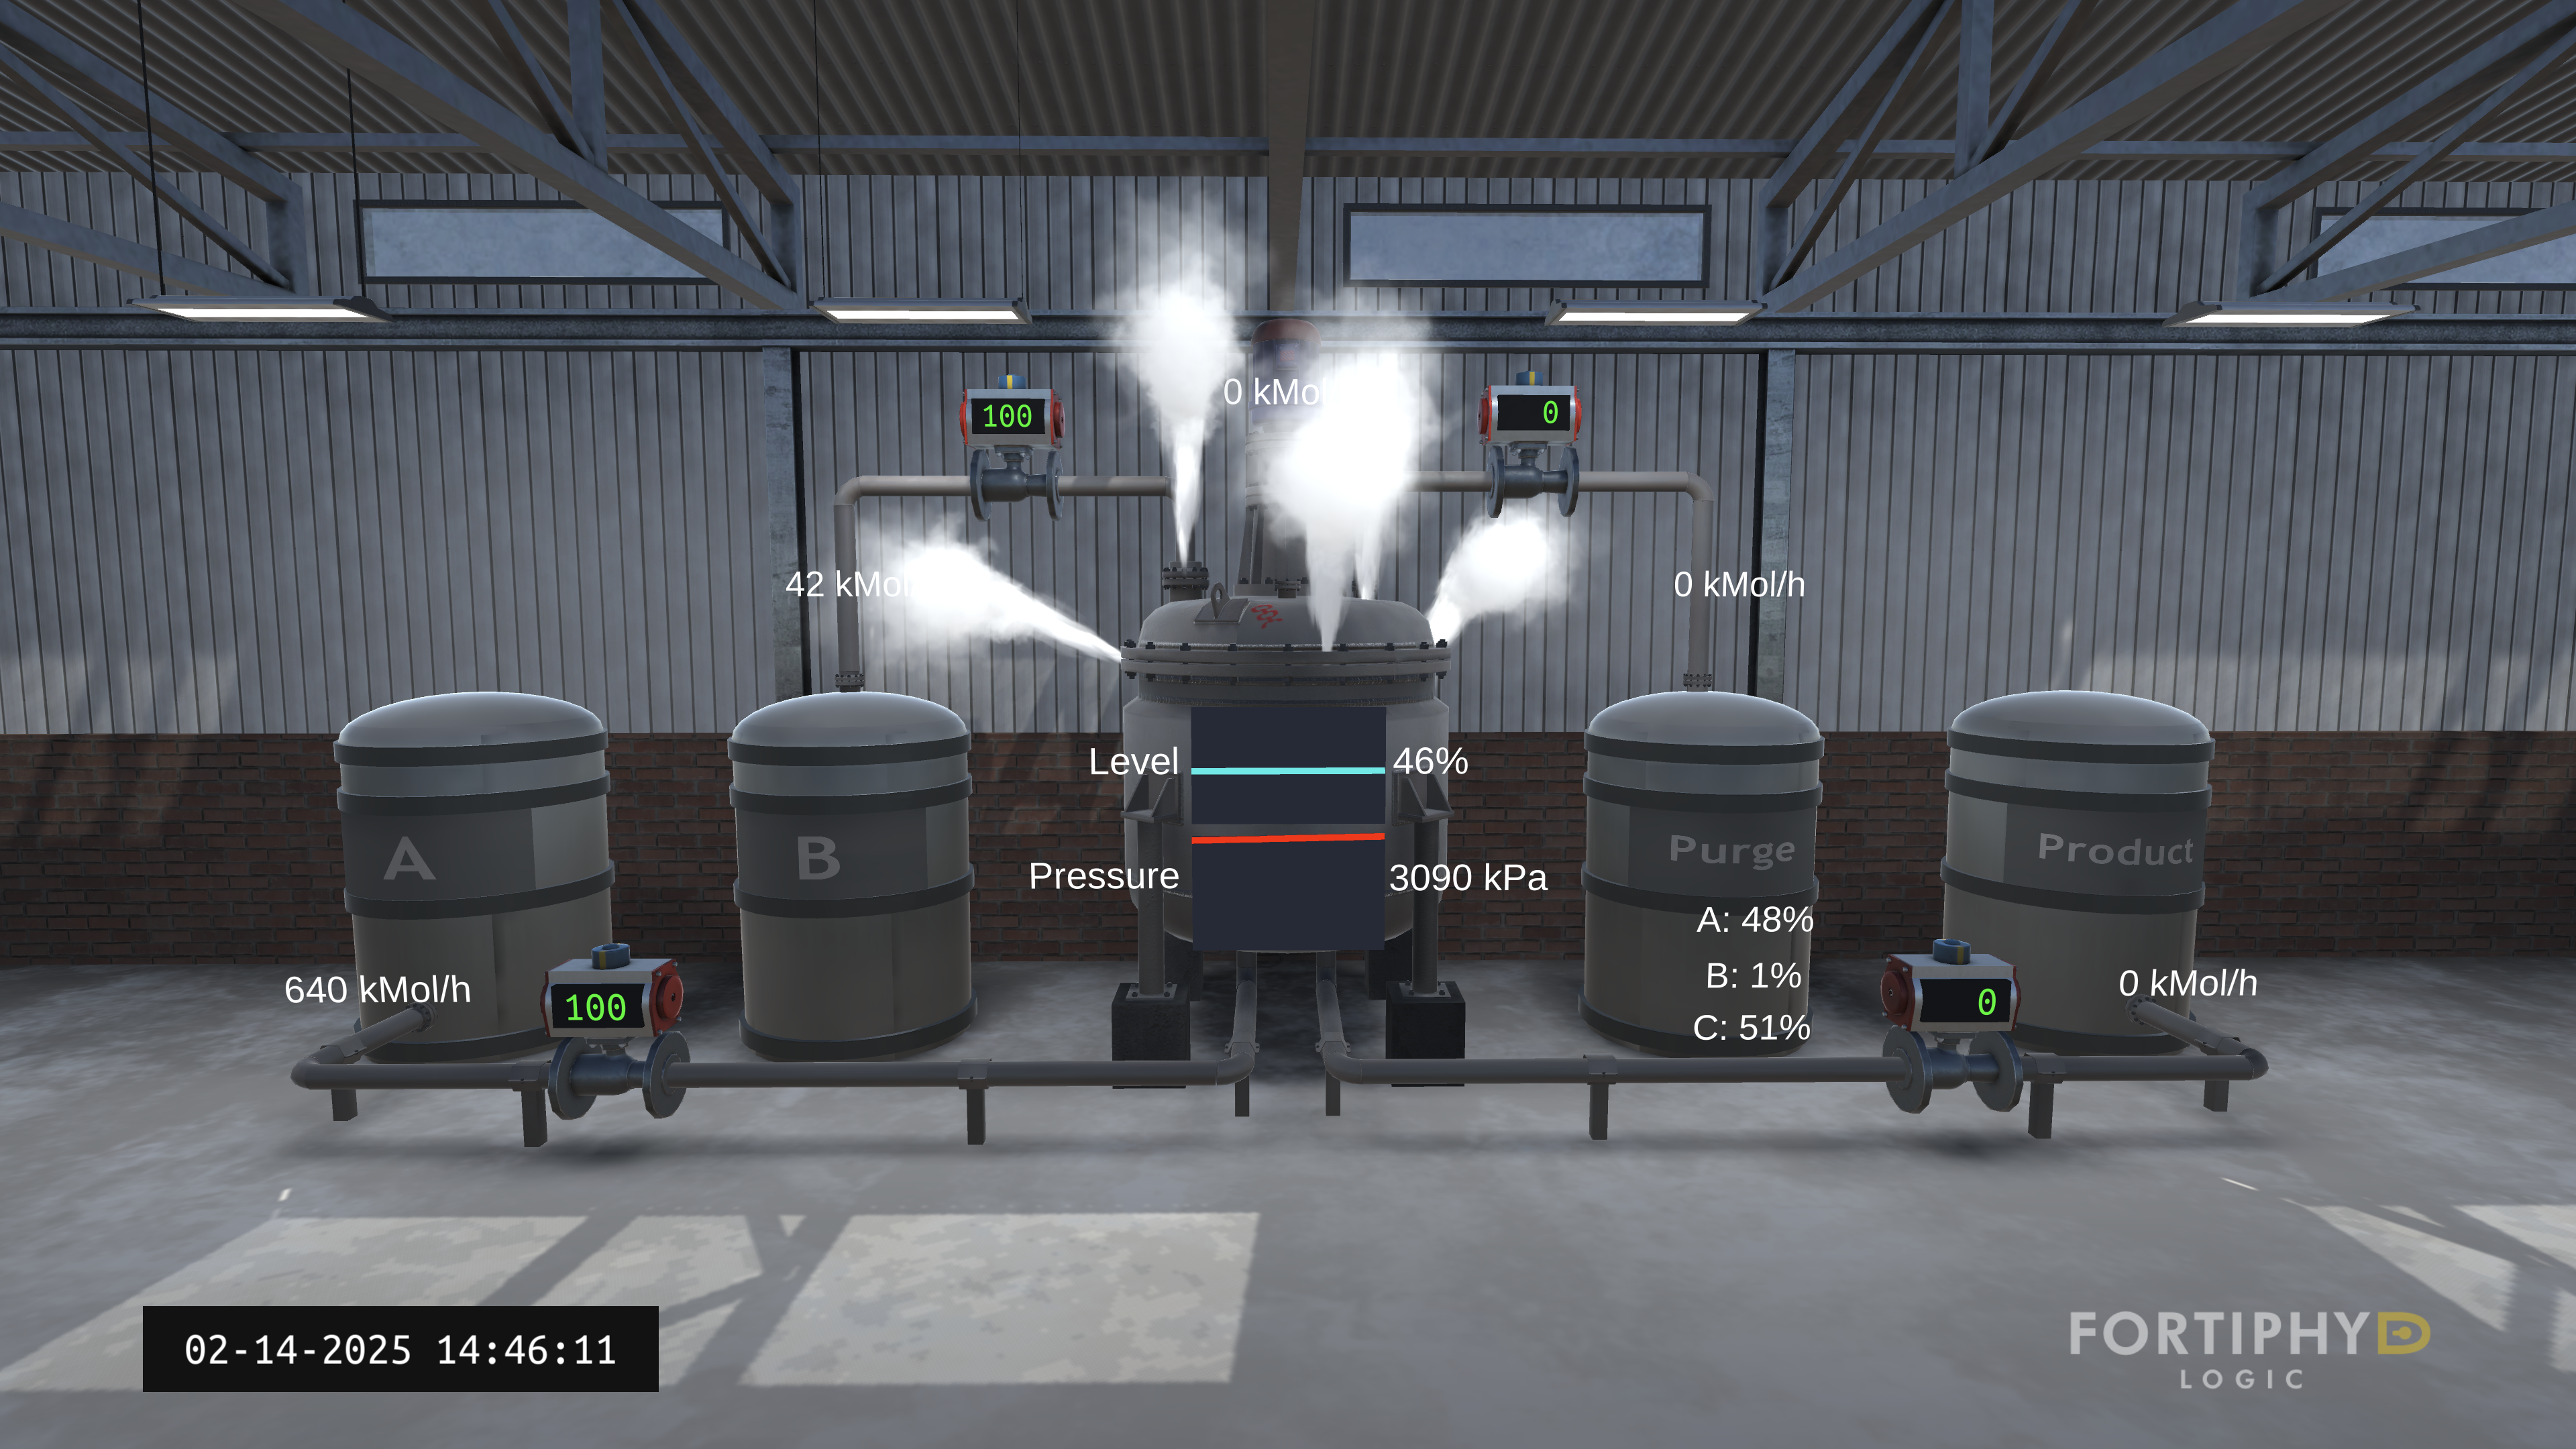
\includegraphics[width=\linewidth,keepaspectratio]{Figures/Stage_3.png}
        % \caption{}
        \label{fig:Stage_3}
    \end{subfigure}
    \hfill % This ensures that there is no additional space between subfigures
    \begin{subfigure}{0.49\linewidth}
\centering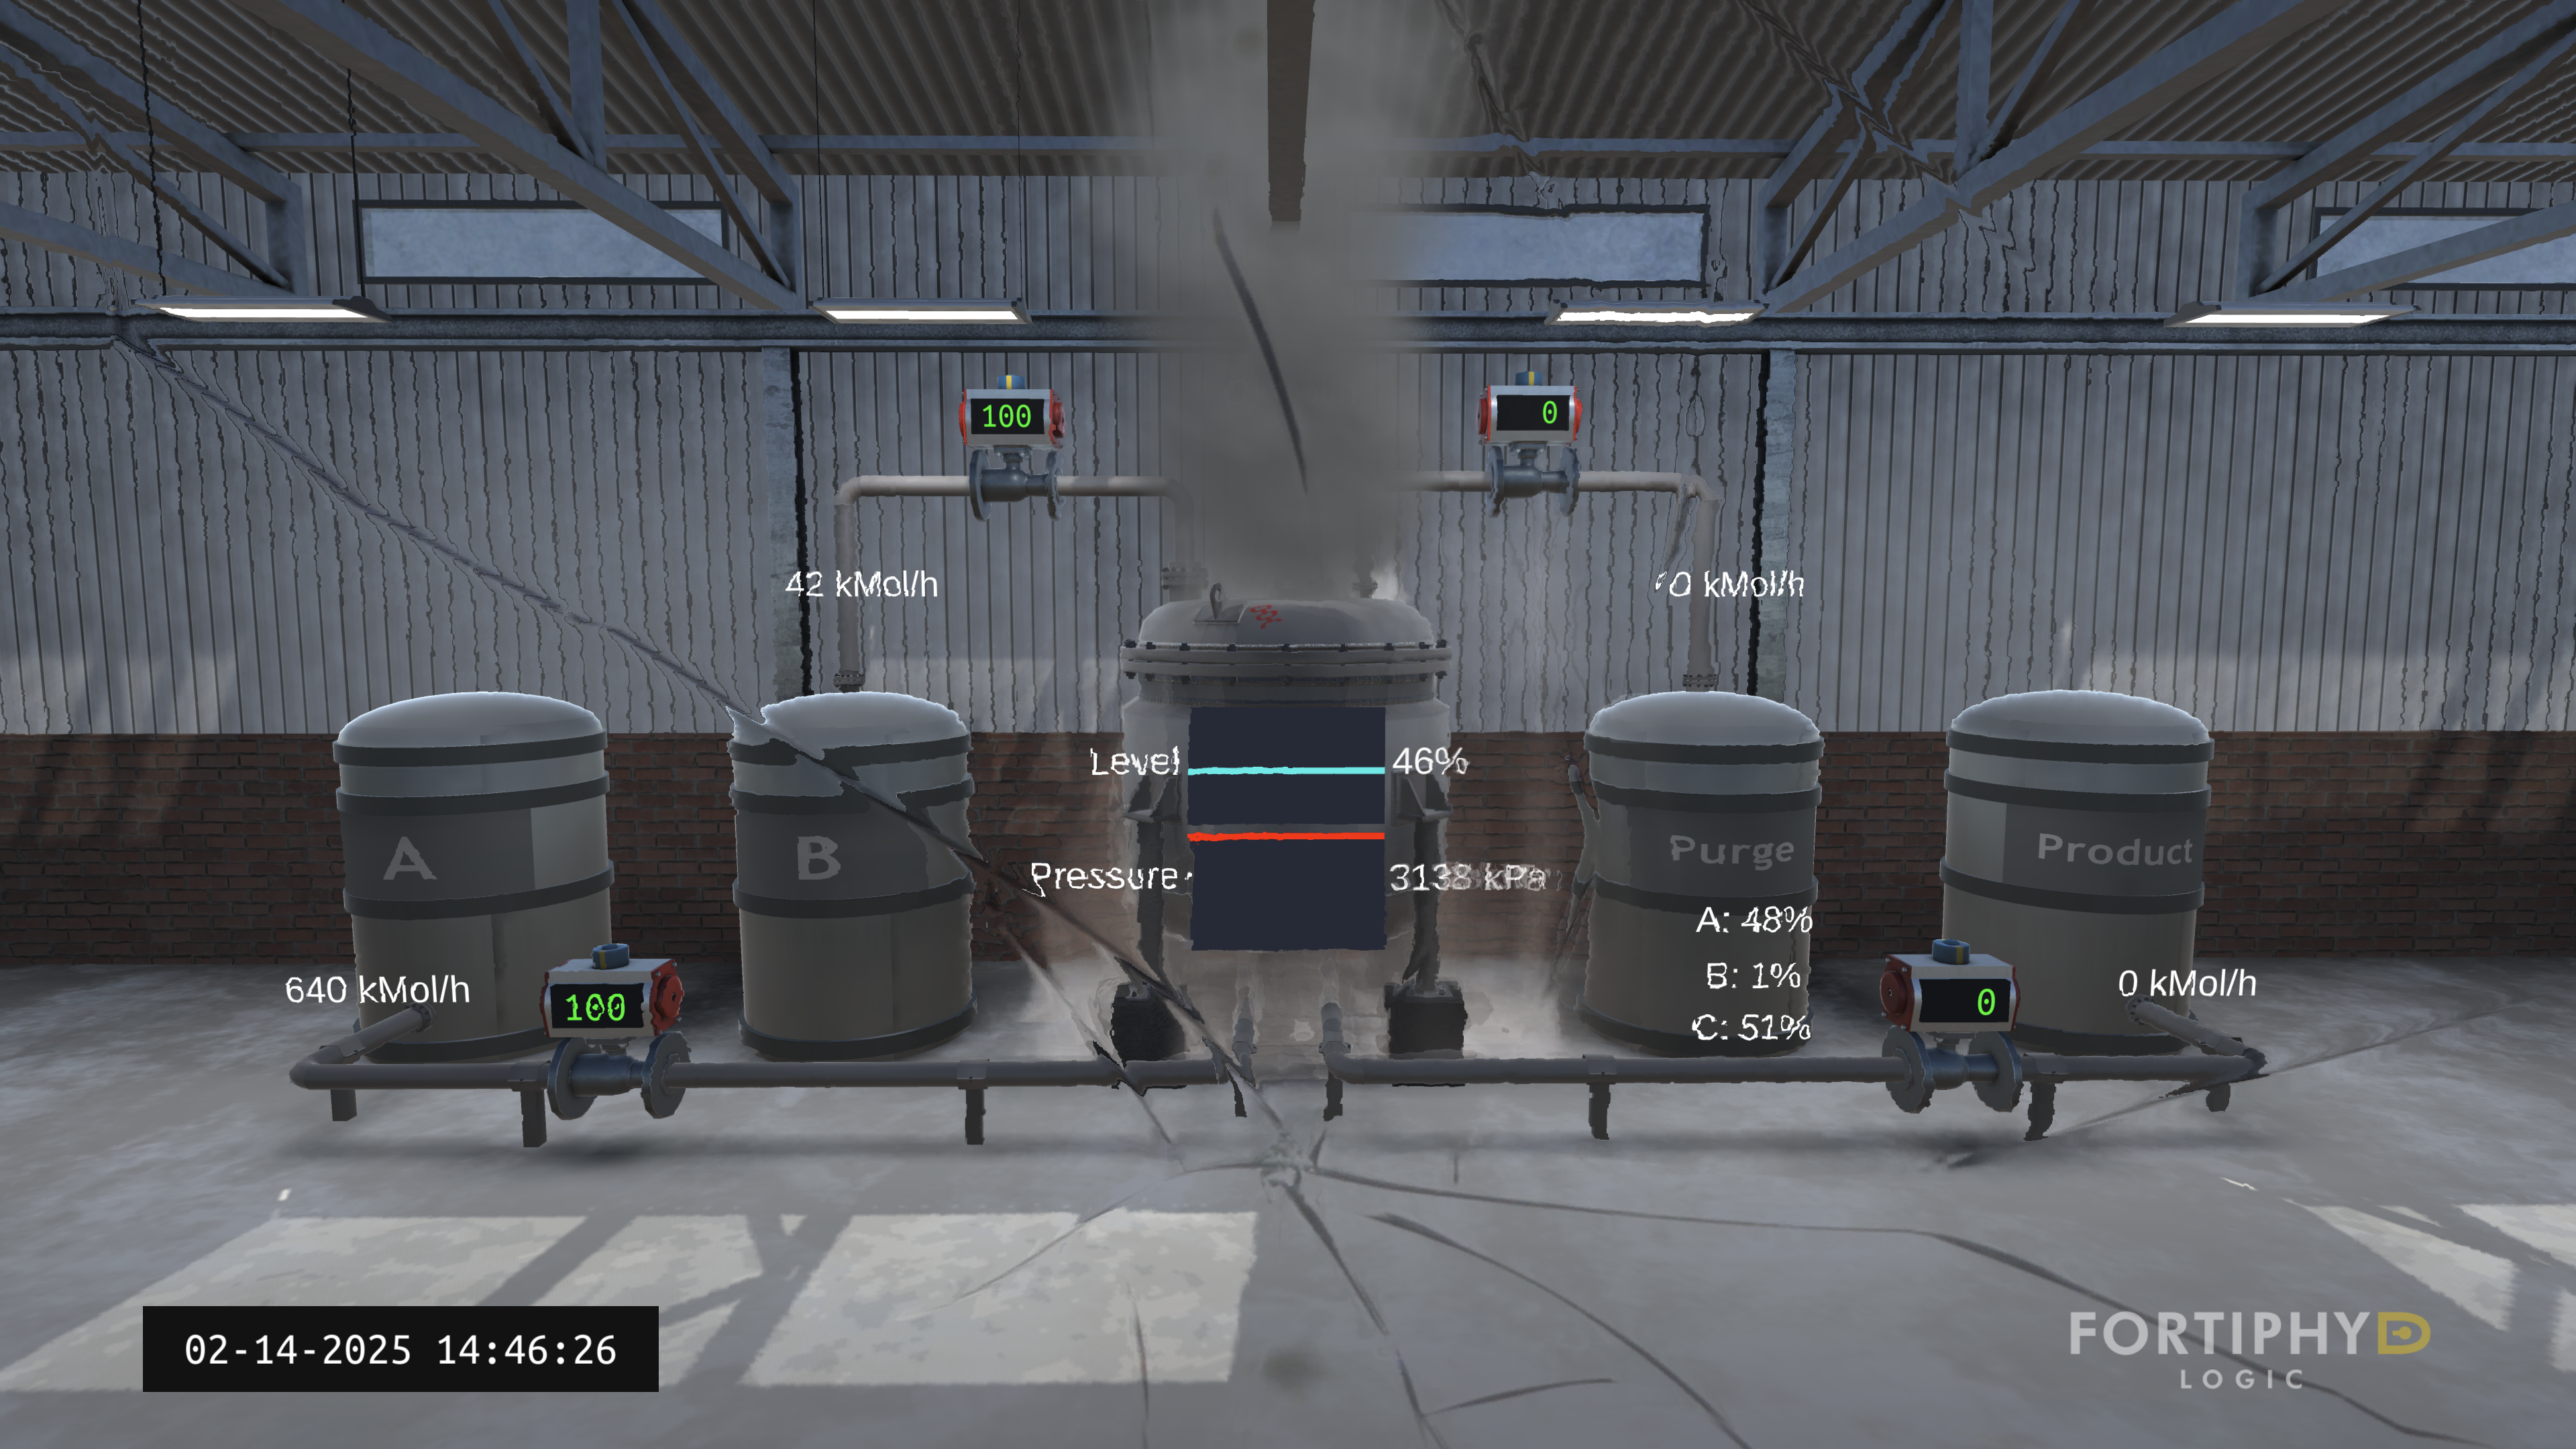
\includegraphics[width=\linewidth,keepaspectratio]{Figures/Stage_5.png}
        % \caption{}
        \label{fig:Stage_5}
    \end{subfigure}
    \begin{subfigure}{\linewidth}
%     \vspace{-0.25cm}
        \centering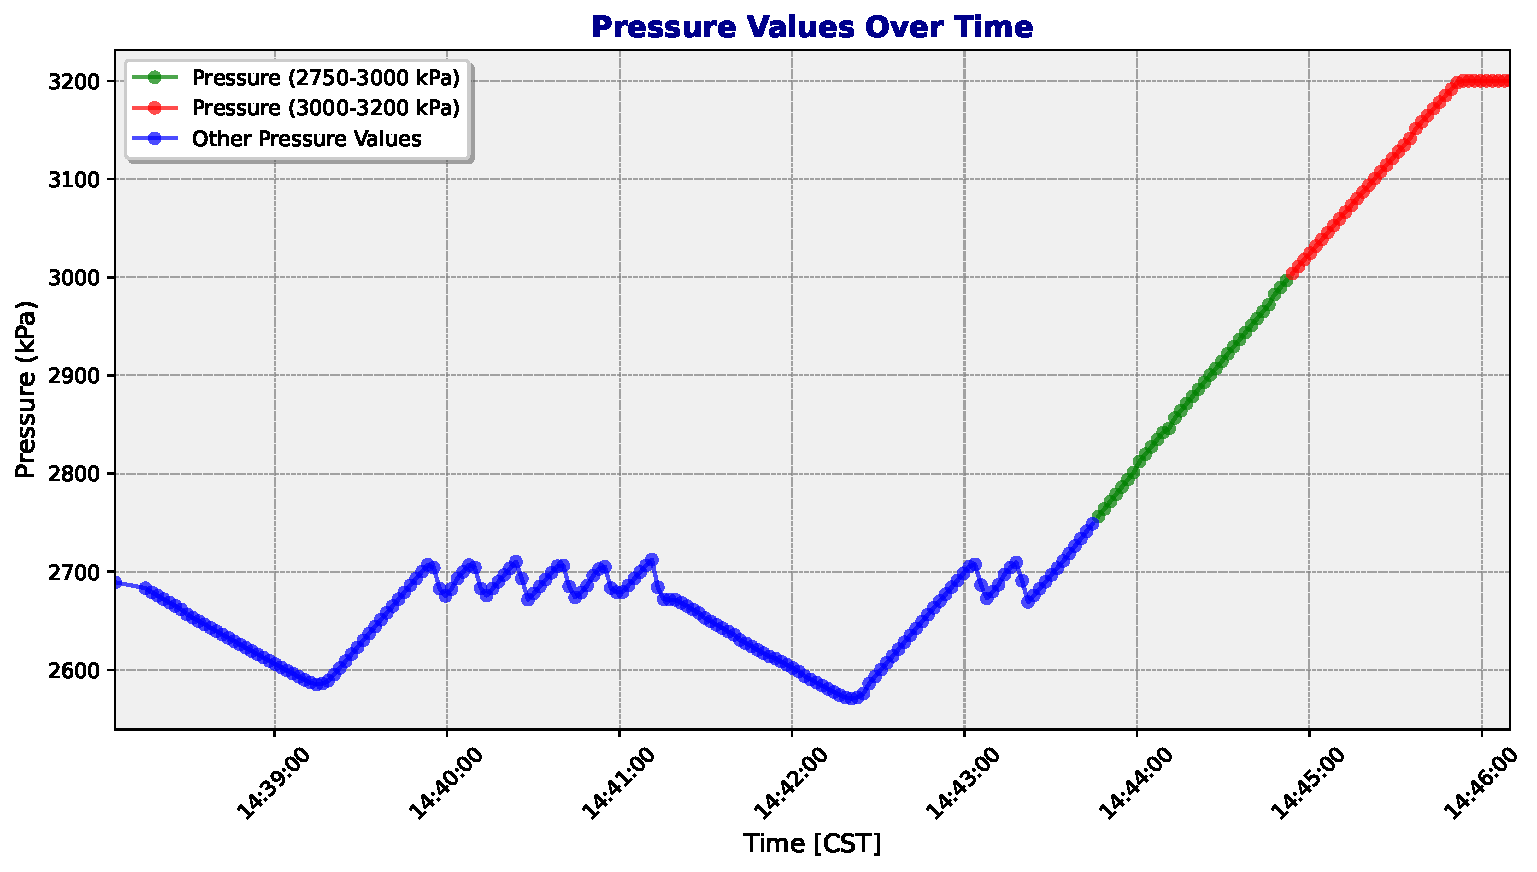
\includegraphics[width=\linewidth,keepaspectratio]{Figures/pressure_plot.pdf}
        % \caption{}
        \label{fig:pressure_plot}
    \end{subfigure}
%     \vspace{-1.25cm}
    \caption{Two different stages in the chemical plant attack emulation showing the instability leading to unavailability of the service. This corresponds to the green and red regions respectively in the pressure plot recorded at the Operator.}
%     \vspace{-0.3cm}
    \label{fig:Chem_figs}
\end{figure}

As described before, the OpenPLC registers hold the values of the setpoint corresponding to different controlled variables of the chemical plant. This control is achieved by regulating the position of the reactants, product, and purge valves based on the user-defined setpoints. The images used in the testbed is set to run the chemical plant at stable values of variables including tank pressure which is set at 2700KPa. There is also a fail-safe value for the pressure beyond which the tank pressure is not allowed to increase which is kept at 2750KPa. These values are written in the registers of the OpenPLC using the SCADA, from where the deployed control algorithm reads and then execute the corresponding control action. We manipulate these setpoints, including the tank pressure, to values higher than the recommended limits. These values are directly written inside the PLC registers, from where the PLC reads it for decision making, thereby taking corrective actions to make the controlled variable reach the desired values. This will cause an increase in pressure and is fatal if left unattended. These changes can be observed from the operator server, where the chemical plant variables are being recorded including the tank pressure. Figure \ref{fig:Chem_figs} shows various stages of the plant before the service unavailability happens.

To understand the effects of DoS attack, we forcefully stop some of the services inside the chemical plant that reports important plant information to the master PLC. We interrupt specifically the Modbus services reporting the measurements of pressure and feed flow (which is a necessary feedback), upon which the controller continues executing the last control action till the desired value is reached. This situation leads to instability due to  the absence of critical feedback, which increases the reaction inside the tank and pushes the pressure beyond safe values. 
% This can be fatal, if the last control action aimed at opening of the feed valves to increase the reaction. 
% In that case, the reaction  will increase inside the tank, making the pressure values go up and thereby pushing the chemical plant to instability. 
The data collected, as shown in the Figure \ref{fig:Chem_figs}, at the Operator server, can help understand the effect of this attack on the Chemical Plant.









\section{Conclusion \& Future Work}
\label{sec:conclusion}

Cybersecurity agents deployed against adversaries require granularity in their actions for informed decision-making to make any network topology resilient. With the advancement in network security, it is important that advanced testbeds are provided where an RL agent can be tested and evaluated. In this work, we aim to provide a testbed for evaluating an agent's policy while dealing with an industrial OT network. With seamless integration of the proposed testbed with any OpenStack network topology, this testbed offers a real-world interface where a trained agent's policy can be evaluated by observing OT-specific observations in addition to the network parameters. With the support from open-source emulators, this testbed can be hosted on any Linux platform provisioned with networking privileges. The installation instructions along with the software requirements are published on our \href{https://github.com/CASTLEGym/OT-Networks.git}{GitHub repository}.

Future work focuses on making the OT workflows discussed in this paper more realistic by adding granularity at the user level. This can open more variables for the users to observe and control, thereby improving the action and observation space of the cybersecurity agents. We are also working on migrating the Power grid OT network to a multi-host, subnet upon replacing Mininet. In addition, we are developing additional OT use-cases with the existing workflows (available in the repository) with various scenarios for users to deploy and evaluate cyber agents.
\subsection*{Acknowledgments}
This material is based on research sponsored by DARPA under agreement number HR001124C0425. The U.S. Government is authorized to reproduce and distribute reprints for Governmental purposes notwithstanding any copyright notation thereon. The views and conclusions contained herein are those of the authors and should not be interpreted as necessarily representing the official policies or endorsements, either expressed or implied, of DARPA or the U.S. Government. We would also like to highlight the efforts by Siemens Corporation, whose initial contributions towards the code base and idea has laid the groundwork for this testbed.


% \newpage
\bibliographystyle{ACM-Reference-Format}
\bibliography{References/references}
% \newpage
\appendices
\onecolumn
% \input{Sections/t10AttackLib}

\end{document}
\endinput
